\documentclass[a4j,12pt]{jarticle}
\usepackage{url}
\usepackage{epsfig}
\usepackage{tabularx}
\usepackage{slashbox}
\usepackage{comment}
\usepackage{subfigure}
\usepackage{multirow}
\usepackage{listings,jlisting}
%コード貼る用のあれこれ
\lstset{
  basicstyle={\ttfamily},
  identifierstyle={\small},
  commentstyle={\smallitshape},
  keywordstyle={\small\bfseries},
  ndkeywordstyle={\small},
  stringstyle={\small\ttfamily},
  frame={tb},
  breaklines=true,
  columns=[l]{fullflexible},
  numbers=left,
  xrightmargin=0zw,
  xleftmargin=3zw,
  numberstyle={\scriptsize},
  stepnumber=1,
  numbersep=1zw,
  lineskip=-0.5ex
}

\def\subfigcapskip{0pt}

\usepackage{ccaption}
\setlength{\abovecaptionskip}{0pt}
\setlength{\belowcaptionskip}{0pt}
\setlength\floatsep{20pt}
\setlength\abovecaptionskip{10pt}
\setlength\belowcaptionskip{10pt}

\newlength{\leftcolumn}
\setlength{\leftcolumn}{0.40\textwidth}
\newlength{\rightcolumn}
\setlength{\rightcolumn}{0.55\textwidth}

\addtolength{\topmargin}{-.75cm}
\addtolength{\oddsidemargin}{0.18cm}
\addtolength{\textwidth}{2zw}
\addtolength{\textheight}{0.5cm}
\addtolength{\footskip}{-0.8cm}
\setlength{\parindent}{2.5ex}
\newcommand{\normaldefault}[1]{\default{}{#1}{#1}}
\newcommand{\default}[3]{\frac{#1\,:\,#2}{#3}}

%図が入りやすくなる魔法のコマンド
  \setcounter{topnumber}{9} % 頁上部の最大float数
  \setcounter{totalnumber}{9} % 1頁の 〃
  \setcounter{dbltopnumber}{9} % twocolumn時の頁上部の最大float数
  \renewcommand\topfraction{.9} % 頁上部のfloatで占める最大の割合
  \renewcommand\textfraction{.001} % 1頁のテキスト部の占める最小割合
  \renewcommand\dbltopfraction{.9} % twocolumn時の topfraction
  \renewcommand\dblfloatpagefraction{.9} % twocolumn時の floatpagefraction
%魔法

% \graphicspath{{../image/}}
\begin{document}
\mbox{}
%**まえがき**

%**{表紙}**
\pagestyle{empty}
\begin{titlepage}
    \fbox{\Large 2021年1月7日提出}
      \vspace*{160truept}
    \begin{center}
      \fbox{\Large 修士論文}

      \vspace{20truept}
      \fbox{
        \begin{tabular}{c}
          {\Huge エンタテインメントを用いた}\\
          {\Huge プログラミング初学者の}\\
          {\Huge 学習意欲促進システムに関する研究} 
        \end{tabular}
      }

      \vspace{110truept}

      \fbox{
        \begin{tabular}{c}
          {\Large 指導教員:西田健志 准教授}\\
          \vspace{10truept}
          {\Large 副指導教員:大月一弘 教授}
        \end{tabular}
      }
      \vspace{50truept}

      \fbox{
        \begin{tabular}{c}
          {\Large 神戸大学大学院国際文化学研究科}\\
          \vspace{10truept}
          {\Large グローバル文化専攻情報コミュニケーションコース}\\
          \vspace{10truept}
          {\Large 学籍番号・氏名 198c125c 岡 大貴}
        \end{tabular}
      } 

  \end{center}
\end{titlepage}

\pagestyle{myheadings}                       % 右上にページ

\newtheorem{theorem}{定理}       % theorem
\newtheorem{definition}{定義}

\renewcommand{\thepage}{\roman{page}\,\,\,}  % 英語ページ
\setcounter{page}{1}
\setlength{\baselineskip}{21pt}
\begin{center}
  {\Large エンタテインメントを用いた\\プログラミング初学者の\\学習意欲促進システムに関する研究}\\
  \vspace{20truept}
    所属専攻・コース:グローバル文化・情報コミュニケーション\\
    氏名:岡 大貴\\
    指導教員氏名:西田 健志\\
\end{center}

\section*{内容梗概}

プログラミングが重要視されている昨今では,プログラミングの授業が小学校に導入されるなど,プログラミングの一般教養化が推し進められている.しかしプログラミングを楽しむためにはある程度の習熟を必要とし,学習中に挫折してしまうプログラミング初学者も少なくない.プログラミングの楽しさを実感させるための初学者向けプログラミング学習コンテンツも存在するが,その多くは小・中学生を対象として設計されておりそれ以上の年代に対しては効果が薄い場合がある.またビジュアルプログラミング言語を用いているため,実践的なテキストプログラミング言語とは乖離がある場合もある.


そこで本研究では初学者のテキストプログラミング言語を用いた学習・興味喚起を促すため,2つのアプリケーションを開発した.1つ目はエンタテインメントの要素を取り入れることによりコードリーディングを促進するソースコード閲覧システムである.このシステムではクイズ,占いといったエンタテインメントを交えてGitHubにあるソースコードを表示し,ユーザが読解それを読み解くことにより,楽しみながらコードリーディングを促進することを目指した.実装したアプリケーションを使用し運用を行い,その後アンケート調査・ディスカッションを行った結果,クイズに関しては楽しかったという回答が得られたが,ややプログラミング初学者にとっては難解であるという意見が得られた.また表示するソースコードを選択するアルゴリズムの改善や,日常的な使用を促すために更なる工夫が必要であり,これらの問題点を今後改善し,より多くの初学者を対象にワークショップ等を行う予定である.


2つ目はリアルタイム性・アドリブを取り入れた対人形式のプログラミングゲームである.このシステムでは習熟度の高いプログラマ2人がプログラミングスキルによって力量を競って勝負することができ,プログラミング初学者でも観戦して楽しむことができる.このゲームの観戦によってプログラミングへの好奇心を高めるとともに,習熟したプログラマへの憧れを創出することで,初学者のプログラミングに対する興味関心を高めることを目指した.評価実験では実際に2人のプログラマの対戦を初学者に観戦させ,プレイヤであるプログラマと観戦した初学者の双方にアンケート調査を行った.実験結果としてゲームのプレイ・観戦は楽しく,プログラミングに対する興味が高まったなどシステムに対する肯定的な意見が多く得られたが,ゲームシステム・デザインの改善点に関するコメントも多く得られた.またプログラマがプレイ時に記述したプログラムを分析した結果,戦略の多様化・より可読性の高いプログラムの表示などいくつかの改善点が見つかった.

この結果を受け,今後は提案システムを改善すると共に,より多くのプログラミング初学者を含むプログラマにシステムを使用させ,より良いシステムの構築を目指す.

\newpage
\markright{}
\tableofcontents            %  目次
\markright{}
\newpage

%###################### 本文 #######################
\renewcommand{\thepage}{\arabic{page}\,\,\,}  % 数字ページ

\setcounter{page}{1}
\setlength{\baselineskip}{19pt}

\newpage
\section{はじめに}

高速にIT化の進む近年では,IoT,AI,クラウドコンピューティングといった単語がメディアで散見されるようになり,誰もがスマートフォンを持ち,TwitterやYouTubeなどのソフトウェアを利用するようになった.家電や自動車,学校教育にもコンピュータが導入され,コンピュータが着実に人々の生活を満たしつつあるといえる.コンピュータが遍在する現代において,人とコンピュータの接点は圧倒的に多くなり,コンピュータを専門的に扱う人でなくともそれに触れて暮らすことが当たり前となっている.就労などの社会活動においても,あるソフトウェアを使いこなせたり,プログラミングができるなどコンピュータとの親和性が高いことがアドバンテージとなる場合もある.

近年ではその高速な社会のIT化に伴い,プログラミングが重要性を増している.国際的には,ロシアでは2009年からプログラミング教育が導入され,英国では2014年から「Computing」というコンピュータサイエンス,情報技術,デジタルリテラシーの3分野からなる科目が導入されており\cite{survey},日本においても今年度から小学校でのプログラミング教育が必修化されている\cite{guide}.以前は「プログラミングはエンジニアや理系の学生がやるもの」というような,専門家だけの技能であるという認識が強かったが,プログラミングが英語のように一般教養となり,プログラミングに関わる仕事に就かない人もある程度理解していることが求められている.

% プログラミングという行為はコンピュータを活用し,ソフトウェア開発・ハードウェア制御などにより人々の活動の生産性を高めるだけでなく,自身のアイディアをコンピュータを介して表現する手段でもあり,プログラミングスキルを向上させることは自己表現の可能性を広げることにつながる.近年ではProcessingやopenFrameworks,Arduinoなどの登場により,プログラミングにより創造的な表現を生み出す「クリエイティブ・コーディング」やメイカームーブメントが流行し,コンピュータ・サイエンス等の知識がなくともプログラミングによってものづくりをし,発表できる土壌が整いつつある.

しかしプログラミング教育の現場やその学習教材では,プログラミングの機能にのみ焦点が当たりがちで,プログラミングの「楽しさ」が疎かにされていることが少なくない.プログラミングをする上で楽しさを感じることは,学習の観点からも重要である.松本らによるC言語プログラミングの授業では、学習の楽しさや、プログラミングへの興味が高いほど授業の学習率が高いことが示されている\cite{matsumoto}.

しかし最初から理解が容易で楽しさを感じやすい読み書きや運動とは異なり,プログラミングは楽しさを感じるまでにある程度の習熟を要する.よく書かれた小説などの文章やプロスポーツでのファインプレーには初心者でも心動かされるもので,そうした小説家やスポーツ選手への憧れが自ら書くことや体を動かすへの感心を高めるが,プログラミングの場合にはそのような憧れをもつ機会に乏しいのが現状である.

プログラミング初学者にプログラミングの楽しさを実感させるために設計された学習コンテンツは多数存在し,ScratchやViscuitなどのビジュアルプログラミング言語(VPL: Visual Programming Language)がその代表的な例である.これらは実際に学校教育で導入され,小・中学生のプログラミング教育に貢献している.しかしそれらは小・中学生など若い年代をターゲットに設計されているため,高校生や大学生,それ以上の年代にとっては楽しさを感じにくい場合がある.また実践的なソフトウェア開発においてはテキストプログラミング言語(TPL: Textual Programming Language)を用いる場合がほとんどであるため,VPLとTPLの間に乖離があることも問題である.

本研究では従来のシステムがターゲットとしている世代よりも上の世代のプログラミング初学者を対象に,エンタテインメントの要素を用いることでプログラミングに対する抵抗感を減らし,プログラムを書かずともプログラミングを楽しんでもらうためのシステムの開発を目指した.具体的には初学者のコードリーディングを促進するアプリケーション,プログラミングゲームを用いてプログラミングに対する興味喚起を行うアプリケーションの2つを開発し,それぞれ初学者を対象に運用を行うことでその効果を検証した.


本論文では以降,2章で研究指針について述べた後,3章でゲーミフィケーションを用いたコードリーディング促進システムについて述べ,4章でプログラミング初学者の興味喚起を目的としたプログラミングゲームについて述べる.5章で本論文をまとめる.
\markright{}

\newpage
\section{研究指針}

本研究の目的は,エンタテインメントの要素を用いてプログラミング初学者のプログラミングに対する抵抗感を減らし,プログラミングを楽しんでもらうことである.


初学者向けプログラミング学習システムの目的は多様であり,プログラミングスキルを向上させることだけでなく,論理的思考力を養うこと,プログラミングに対する興味関心を高めることなど様々である.例えばScratchはプログラマの育成ではなく,自分の考えを表現するための手段・思考としてプログラミングを教えるために設計されており,Viscuitは子供や情報処理の専門家を目指さない大人に対して,プログラミングの楽しさを伝えるために設計されている.

本研究ではVPLではなくTPLによって実践的なプログラミングへ初学者を向かわせるとともに,その楽しさを感じさせることを目指す.


初学者がプログラミング学習を挫折してしまう要因はいくつか考えられるが,本研究ではそのうち3つの要素に焦点を当てた.

1つは「辛さ」である.プログラミング初学者向け教材では,記述されているプログラムを書き写す,いわゆる「写経」を行い,サンプルアプリケーションの作成などをする.これは学びの多い作業ではあるが,単調な作業になり,初学者にとっては苦痛を伴う場合がある.


2つ目は「煩わしさ」である.初学者が挫折する原因として多いのが環境構築が上手くいかず,学習を諦めてしまうことである.また特にコンピュータを日常的に使用する習慣がない場合はプログラミングから遠ざかりがちである.


3つ目は「難しさ」である.プログラミング学習と言ってもその内容は多岐に渡り,あるプログラミング言語の文法だけでなくオブジェクト指向等の概念やライブラリ,エディタ,IDE,VCS等ツール群の用法など多くを学ばなければならない.初学者にとって難解な概念も多く,これらを並行して学ぶことはモチベーションを下げかねない.

上記の問題を解決するため,以下の指針を設けた.開発するシステムにはこれに基づいた設計指針を設ける.

\begin{enumerate}
  \item {\bf エンタテインメントの要素を取り入れる}

  コンピュータを日頃使わない者にとって,プログラミングに触れる機会は少ないため,初学者はプログラミングをすることあるいはプログラムを読むことに慣れておらず,少なからず抵抗感があると考えらえる.本研究ではエンタテインメントの要素を取り入れることで,プログラムに触れることへの抵抗感を減らすとともに能動的な利用を促し,プログラムに触れることを楽しんでもらうことを目指す.

  \item {\bf 利用のハードルを下げる}

  初学者にとって環境構築や,普段使用しないソフトウェアの導入などの手間は,プログラミングに対するモチベーションを下げる要因となる.本研究ではシステムを利用する際の手間を極力小さくすることで,日常的な利用を促進し,初学者がプログラミングと接する機会を増やすことを目指す.

  \item {\bf 不要な負荷をかけない}

  複雑な概念や理解が何回な要素は初学者の挫折の要因である.本研究では極力前提知識などを少なくし,初学者がプログラムあるいはプログラミングのみに集中できるように設計する.
\end{enumerate}

研究指針と設計した各システムでの設計指針の関係を表\ref{research_guidelines}に示す.

\begin{table}[ht]
  \centering
  \caption{各システムでの設計指針}
  \label{research_guidelines}
    \begin{tabular}{|c|c|c|} \hline
      研究指針 & コードリーディング支援システム & プログラミングゲーム  \\ \hline\hline
      遊びの要素を取り入れる & クイズ・占いを用いる & 
      \begin{tabular}{c}
        駆け引き・アドリブを\\取り入れる
      \end{tabular}\\ \hline
      利用のハードルを下げる & 日常的に使用するツールに組み込む & 見て楽しめる\\ \hline
      不要な負荷を書けない & プログラムを読むことに専念させる & 専門知識を必要としない \\ \hline
      
    \end{tabular}
\end{table}

\newpage
\section{コードリーディング支援システムの開発}

本項では,プログラミング初学者を対象としたコードリーディング支援システムについて紹介し,設計指針に基づくデザインの詳細,プロトタイプを用いたケーススタディとその後に開発したWebアプリケーションについて説明する.

\subsection{研究背景}
プログラミングの重要性の高まりに伴い,コンピュータに関連する分野を専攻していなくとも,プログラミングを独学で学ぼうとする人が増えている.そういった人はプログラミング学習用書籍やWebサイトを通して学ぶ場合が多い.初学者向けプログラミング学習コンテンツが普及し,プログラミングに入門するハードルは下がってきているものの,まだプログラミングを独習できる環境が整っているとは言えない.

プログラミング学習において重要とされるスキルは数多くあり,自分でアルゴリズムを考え実装する能力だけでなく,情報収集能力,コードリーディングスキルなど様々である.これらをコンピュータについての知識が乏しい者が独習するのはハードルが高い.初学者向け学習教材においては,写経型学習を主とし,プログラムを「書く」技能を磨かせるものが多い.プログラミング学習サイトであるProgate\cite{progate}では,主要なプログラミング言語の文法やライブラリの用法など,「どうプログラムを書くか」を重点的に教えている.


しかし学習教材を用いた学習では,コードを「読む」技能,すなわちコードリーディングスキルが培われず,複数人で共同開発し他人の記述したプログラムを読解したり,ライブラリのソースコードにあたる際に苦労が生じる.また初学者向け学習教材では比較的平易なプログラムしか載っていないため,実践的なソースコードに触れ,内容を読解したり,他者のコーディングスタイルから学びを得る機会が生まれ辛い.

本項で提案するシステムでは,コードリーディングスキルに焦点を当て,エンタテインメントの要素を組み込んで初学者に実践的なプログラムを閲覧させることにより,初学者のコードリーディングを促進するシステムを実装した.
\subsection{関連研究}

%GitHub使った研究
\subsubsection{GitHub上のデータを利用した研究}
GitHubを活用した研究はいくつかある.Guzmanらの研究ではGitHub上のオープンソースプロジェクトにおけるコミットコメントから感情分析をし,その結果とプログラミング言語やコミットの時間などとの相関を調査している\cite{guzman}.永野らの研究ではGitHubとStackOverflowのデータを用いて双方を利用するユーザについて調査している\cite{nagano}.この研究ではユーザがGitHubで作成したリポジトリとStackOverflowへの投稿のコンテンツの関連性について調べたもので,双方への投稿コンテンツに一定の相関があることを示している.また柴藤らはGitHub上の断片データに関する情報を取得できるシステムを開発している\cite{shibatou}.このシステムではユーザが指定したソースコード中の一部の連続したコードに関するプルリクエストを取得できるというものであり,ソースコードを閲覧する際の利便性を高めている.これらの研究からGitHubのソースコードやコミットコメントには有益な情報が含まれていることが分かるが,これらを初学者のコードリーディング支援のために活用している例は見かけない.

%エンタテインメント,ゲーミフィケーション使った研究
\subsubsection{ゲーミフィケーションを活用した研究}
またエンタテインメントの要素,特にゲーミフィケーションを活用した研究も盛んである.一ノ瀬らの研究\cite{ichinose}ではソースコード上の技術的負債を可視化し,さらにゲーミフィケーションの要素を加えることで技術的負債の除去を促している.この研究ではソースコードのファイル構造を街のように可視化し,技術的負債が存在するファイルを目立たせ,さらに技術的負債を取り除いたユーザをランキング形式で表示することによって,ゲーミフィケーションの要素を活用し生産的な行動を促している.三谷らの研究\cite{mitani}ではキャラクタをプログラムで制御するプログラミングゲームでプログラミングスキルの向上を図っており,筒井らの研究\cite{tsutsui}ではパズルゲームにより,初学者のオブジェクト指向の理解を深めるシステムを開発している.これらはプログラミングの上達あるいはソフトウェア開発のためにゲーミフィケーションを利用しているが,コードリーディングに着目し,初学者のコードリーディングを促進するためにゲーミフィケーションを利用したシステムは見かけない.

%コードリーディングに関する研究
\subsubsection{コードリーディング支援に関する研究}
なおコードリーディング支援に関してもいくつか研究がなされており,大村らや石尾らはソースコードを読解する際のコードリーディング支援を行うツールを開発している\cite{omura}\cite{ishio}.
しかし,これらの研究ではある程度プログラミングに習熟したプログラマがソースコードを読むという状況を想定しているため,初学者に向けコードに触れる機会を増やすための工夫は成されていない.
\subsection{設計指針}
システムを実装するにあたり,研究指針に基づいた3つの設計指針を設けた.
\begin{enumerate}
  \item {\bf クイズ・占いを用いる}

  コードリーディングはプログラミングにおいて重要なスキルの1つであるが,プログラムを読解した経験の少ないプログラミング初学者にとって,淡白なプログラムをただ読み込むことは心理的ハードルが高い.よって本システムではクイズ・占いといった誰もが知っているエンタテインメントの要素を付与してプログラムを読解させ,コードリーディングの心理的障壁を下げることを目指した.


  \item {\bf プログラムを読んで楽しめる}


  本項で述べるシステムの目的は,初学者のコードリーディングを促進することである.プログラムを「書く」ことに焦点をおいた教材は他に多く存在するため,本システムではプログラムを「読む」ことのみに専念させ,余計な認知的負荷をかけずに読解に集中できるように設計する.また1つのプログラミング言語を読解するだけでなく,様々なプログラミング言語に触れることで,コンピュータを取り巻くプログラミング言語とそのライブラリ,エコシステムなどに触れ,プログラミングに対する興味関心を高めることが可能であると考え,1つのプログラミング言語のみを対象とした機能と様々なプログラミング言語に触れる機能を用意した.


  \item {\bf コミュニケーションを創出する}
  初学者がプログラミングを独習する場合,プログラミングを学習している者とのコミュニケーションが発生しづらく,モチベーションが下がる場合がある.本項で提案するシステムでは,エンタテインメントの要素を用いるだけでなく,プログラミングに関するコミュニケーションを創出し,楽しく継続的なシステムの利用を促す.
\end{enumerate}

\subsection{提案システム}
\subsubsection{実装機能}
提案システムに実装する,エンタテインメントの要素を用いた2つの機能について説明する.
\begin{itemize}
  \item {\bf クイズ機能}

  この機能はユーザが使用した際にGitHubからランダムに取得したプログラムを表示する.プログラムの記述言語は多様であり,ユーザは表示されたプログラムを読み,どのプログラミング言語で記述されたプログラムかを回答する.正解した場合は得点が得られ,取得した累計得点の多さによるランキングが表示される.設計指針2で述べた様々な言語に触れられる機能に相当する.

  \item {\bf 占い機能}

  この機能をユーザが使用するとGitHubからランダムに得られたプログラムが表示され,ユーザはそれを読解し自分なりの解釈をすることで,その日の運勢を占う.表示されたソースコードの意味を解釈することが必要であるため,必然的にコードの読解が必要となる.この機能においては表示されるプログラムをJavaScriptで記述されたものに限定した.

\end{itemize}

\subsection{プロトタイプシステム}
初めに,提案システムをチームコミュニケーションツールであるSlackのbotとして実装した.システムを利用する際は,このbotを導入しているチャンネルでコマンドを入力することで各機能を使用できる.利用可能なコマンドを表\ref{function}に示す.

また表示するプログラムは内容が1つのファイルにまとまっていることが望ましいため,GitHub Gistからプログラムを取得した.クイズ機能を使用している様子を図\ref{prototype_quiz}に,占い機能を使用している様子を図\ref{prototype_fortune}に示す.

\begin{table}[!ht]
  \centering
    \caption{コマンド一覧}
      \begin{tabular}{|c|c|} \hline
        コマンド & 説明 \\ \hline \hline
        fortune & 1日の運勢を占うソースコードを表示 \\ \hline
        quiz & 記述言語を問うクイズを出題 \\ \hline
        hint & クイズに関するヒントを表示 \\ \hline
        answer & クイズの回答を表示 \\ \hline
        score & 各ユーザの累計得点を表示 \\ \hline
      \end{tabular}
    \label{function}
  \end{table}

\begin{figure}[!h]
  \begin{center}
    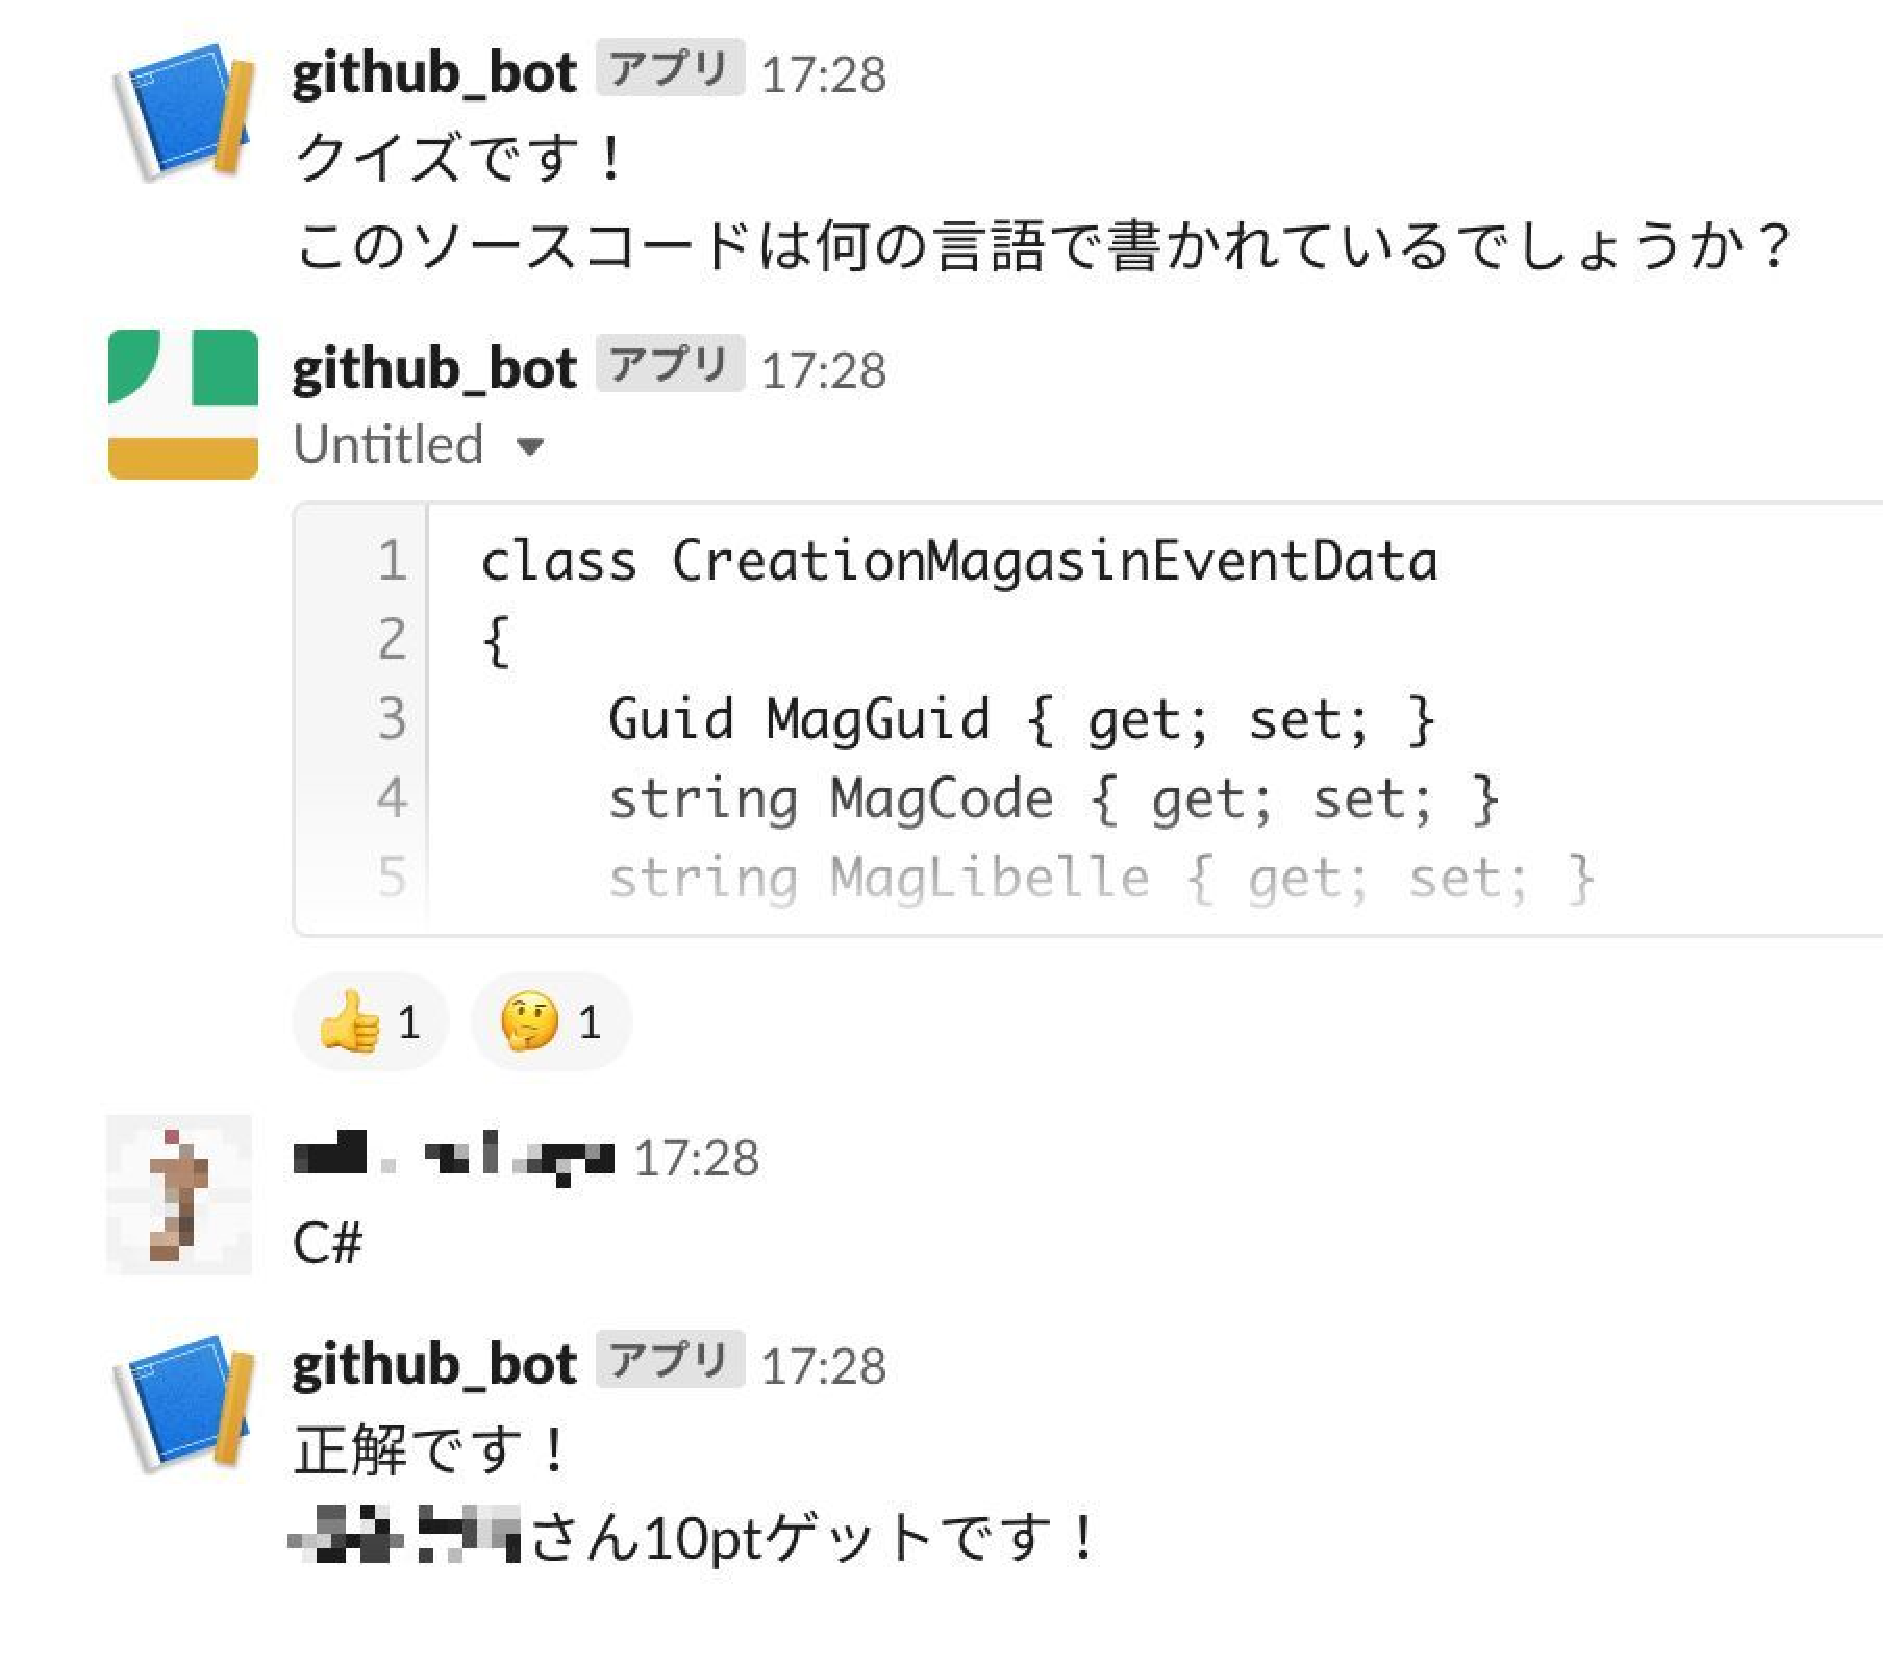
\includegraphics[width=0.4\linewidth]{image/prototype_quiz.eps}
  \end{center}
    \vspace{-8mm} 
  \caption{クイズ機能の様子}
  \label{prototype_quiz}
\end{figure}

\begin{figure}[!h]
  \begin{center}
    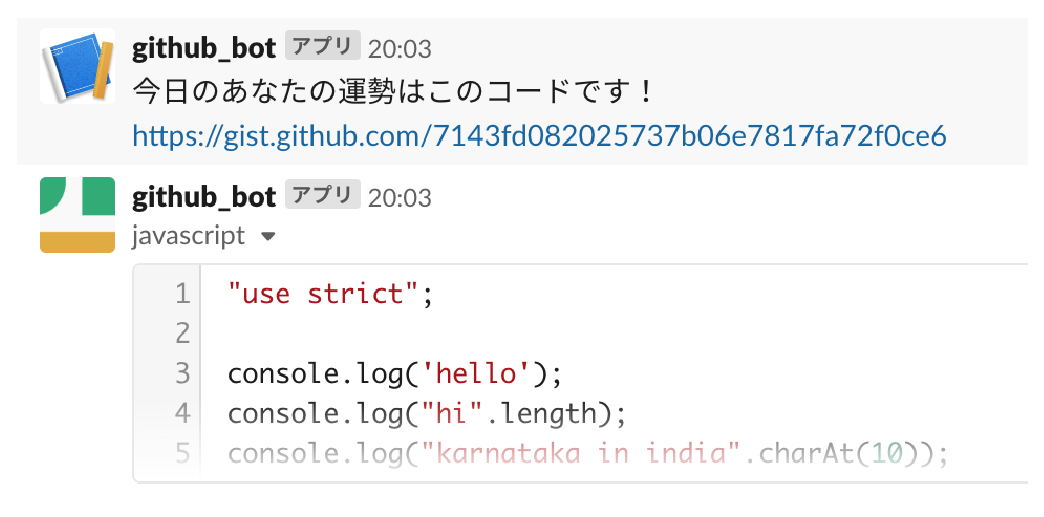
\includegraphics[width=0.6\linewidth]{image/prototype_fortune.eps}
  \end{center}
    \vspace{-8mm} 
  \caption{占い機能の様子}
  \label{prototype_fortune}
\end{figure}


\subsubsection{ケーススタディ}
このシステムを筆者が所属する研究室で運用しているSlackのチャンネルに導入し,システムの効果を調査するため,研究室のメンバーを対象としたケーススタディを行った.研究室のメンバーは3名のプログラミング初学者であり,主にJavaScrtipやGoogle Apps Scriptを使用している.ケーススタディの内容としては,1週間自由に機能を使用してもらい各コマンドの使用回数を調べ,アンケートによって所感を調査した.アンケートの項目を以下に示す.

\begin{itemize}
  \item どういう状況で機能を使用したか
  \item 占い機能について,楽しかったか(5段階評価,1:楽しくなかった,5:楽しかった)
  \item 占い機能について,どういう点が楽しかった(楽しくなかった)か
  \item クイズ機能について,楽しかったか(5段階評価,1:楽しくなかった,5:楽しかった)
  \item クイズ機能について,どういう点が楽しかった(楽しくなかった)か
  \item 機能を使用したことによって学びがあったか
  \item どういう学びがあったか
  \item コードを読むことへの抵抗は減ったと感じるか(5段階評価,1:減らなかった,5:減った)
  \item 今後も機能を使いたいか
  % \item 感想,意見,改善点など
\end{itemize}

また各コマンドの使用回数を表\ref{command}に示す.

\begin{table}[!h]
  \centering
  \caption{各コマンドの使用回数}
  \label{command}
    \begin{tabular}{|c|c|} \hline
      コマンド & 使用回数 \\ \hline \hline
      fortune & 9 \\ \hline
      quiz & 43 \\ \hline
      hint & 27 \\ \hline
      answer & 3 \\ \hline
      score & 33 \\ \hline
    \end{tabular}
\end{table}

コマンドの使用回数に関しては,クイズ機能に関連した機能が多い結果となり,占い機能に関しては使用回数が少なかった.なお期間中の最初の3日間ほどは頻繁にシステムが使用されていたが,期間の後半おいてはあまり活発に使用されていなかった.またどの機能も個別に使用するより,ユーザが実際に会って集まっている際にコミュニケーションを交えて使用されることが多く,コミュニケーションを促進できていたと考えられる.

次にアンケート結果を表\ref{interview}に示す.
\begin{table}[!b]
  \centering
  \caption{アンケート結果}
  \label{interview}
    \begin{tabular}{|c|c|c|c|} \hline
      インタビュー内容 & 被験者A & 被験者B & 被験者C \\ \hline \hline
      占い機能は楽しかったか & 1 & 2 & 3 \\ \hline
      クイズ機能は楽しかったか & 4 & 4 & 5 \\ \hline
      コードへの抵抗感は減ったか & 3 & 5 &5 \\ \hline
    \end{tabular}
\end{table}

まず占い機能に関してだが,使用する楽しさの評価は低い結果となった.ユーザの意見には「提示されたプログラムをどう解釈すればいいのか分からなかった」「占いという感触があまりなかった」などがあり,プログラミング初学者にとってプログラムを読解して独自の解釈を持たせることは難しく,面白みに欠けているようだった.

またクイズ機能に関しては楽しさに関して高い評価が得られた.その理由として「スコアがあると、競争している感が出るところが楽しく感じた」「みんなで一緒にやっていて競争っぽくなるとき楽しかった」などの意見があり,スコアを用いたゲーミフィケーション,競争の要素がシステム使用のモチベーションを高めていたと考えられる.

なお「以前に出た言語の特徴に似ていると感じ、調べずに答えて正解したとき楽しかった」という意見が得られ,クイズを通したコードリーディングによってプログラミング言語の特徴を捉え,それに楽しみを感じていることが分かった.

「機能を使用したことによって学びがあったか」という質問には全員が「あった」と回答し,「どういう学びがあったか」という質問には「言語ごとの文法の特徴が何となく分かってきた」「いろんな言語の存在を知ることができました」「今まで聞いたこともなかったプログラミング言語の名前を知り、親近感をもった」という回答があり,各プログラミング言語の特徴について理解するとともにプログラミングに対する親近感を抱かせることができていた.

またプログラムへの抵抗感に関する質問でも肯定的な評価が得られ,「今後も機能を使いたいか」という質問に対して全員が「使いたい」と回答した.なおシステムの改善点に関して「プログラムのあるGitHubのページへのリンクを表示して欲しい」「占いの際にラッキーアイテムなどを表示して欲しい」等の意見が得られたため,アンケート結果を元にプロトタイプを改善したシステムを開発した.

\subsection{Webアプリケーション}
プロトタイプシステムを用いたケーススタディで得られた結果を元に,プロトタイプシステムを改善し,Webアプリケーションとして再実装した.Webアプリケーションとして実装したのはSlack botよりも開けたコミュニティでより多くのユーザの意見を取り入れるためである.

このアプリケーションでは指定のURLにアクセスすることでクイズ・占いの機能を使用でき,ユーザ登録をしログインすることでクイズ正解時に得た得点の累計によるユーザのランキングを閲覧することができる.またクイズ機能においてはそのクイズに対するユーザの正答率,占い機能においては選ばれたプログラムに含まれているコメントの量,宣言された関数の数などから独自に算出した対人運,仕事運,コメントなどを表示するようにした.クイズ機能の様子を図\ref{quiz}に,占い機能の様子を図\ref{fortune}に示す.

\begin{figure}[H]
  \begin{center}
    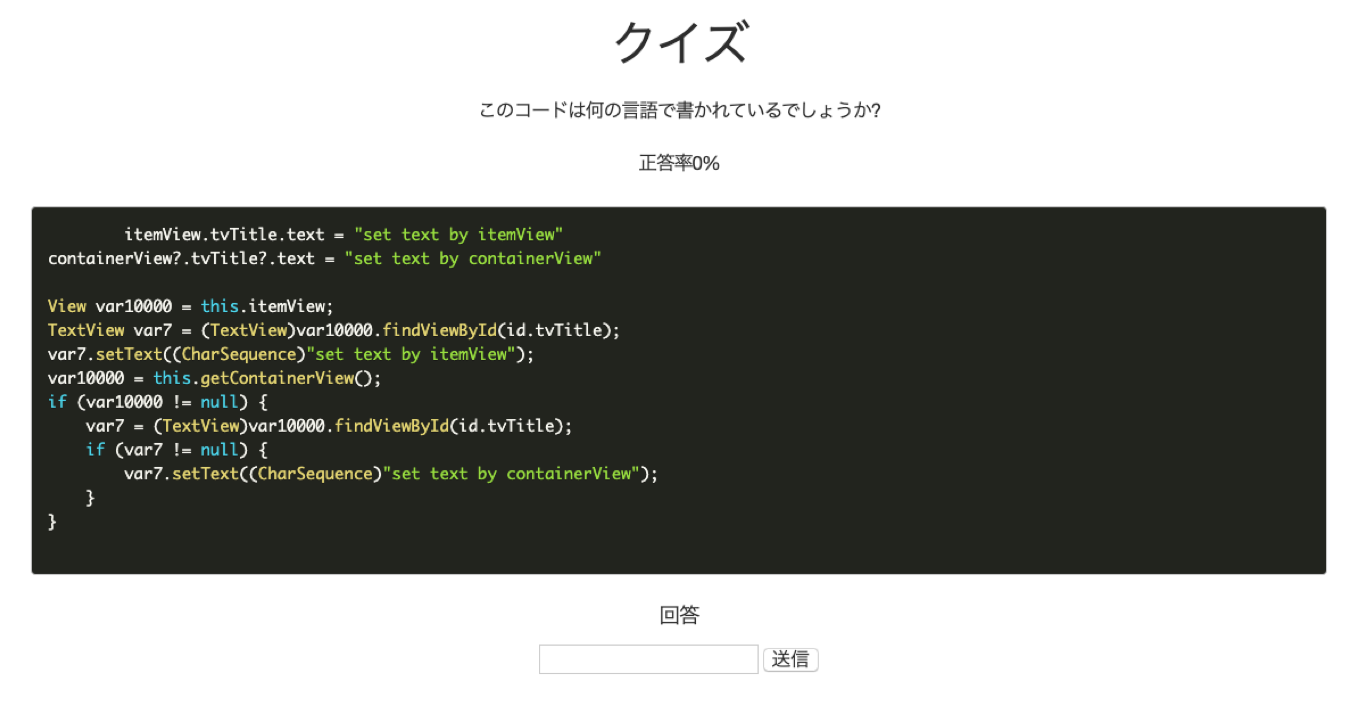
\includegraphics[width=0.8\linewidth]{image/quiz.eps}
  \end{center}
    \vspace{-8mm} 
  \caption{クイズ機能の様子}
  \label{quiz}
\end{figure}

\begin{figure}[H]
  \begin{center}
    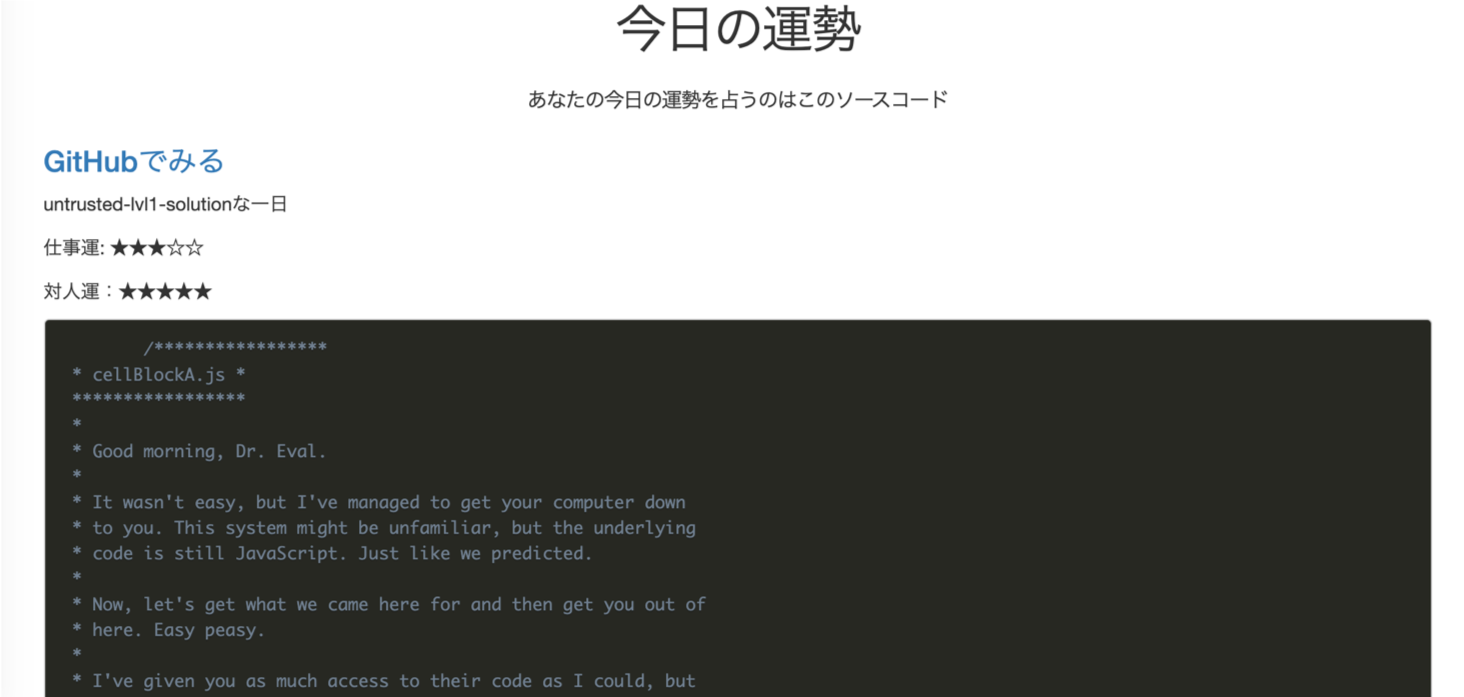
\includegraphics[width=0.8\linewidth]{image/fortune.eps}
  \end{center}
    \vspace{-8mm} 
  \caption{占い機能の様子}
  \label{fortune}
\end{figure}

また実装したアプリケーションをUbiquitous Wearable Workshop2019\cite{uww2019}にて参加者に使用させ,議論を行った.占い・クイズ機能ともに使用され,表示されたプログラムを見せ合うなどシステムを介したコミュニケーションが見られたが,「クイズが難しすぎて逆にプログラムに対する抵抗感が生まれた」というコメントもあった.




\subsection{課題と考察}

提案システムのプロトタイプ及びそれを元にしたWebアプリケーションの実装と運用を通して,エンタテインメントの要素やコミュニケーションの要素,特にクイズの要素を交えてプログラミング初学者のコードリーディングを促進することは,有効な方策であると考えられる.またその中で他者と競争するゲーミフィケーションはシステムを使用するモチベーションとなり,これをプログラミング学習コンテンツに取り込むことで有益な学習コンテンツを作成できると感じた.しかし,現状実装したアプリケーションには不十分な箇所が多く,より適切なゲームデザイン,ユーザがシステムを使い続けるための工夫,どのようなアルゴリズムでプログラムを選び,初学者に提示するかなど課題は多い.

今後はこのシステムを通して得られた課題・観点を元に,より良いプログラミング学習コンテンツを作成していく.またアンケート調査に止まらず,ユーザのコードリーディングに関する行動の追跡的な調査をし,システムに関する客観的な評価を行っていきたい.


\newpage
\section{競技性・観戦性を拡張したプログラミングゲームの開発}
本項では,プログラミング初学者の興味喚起を目的としたプログラミングゲームのプロトタイプについて紹介し,設計指針に基づくデザインの詳細や行った評価実験と見つかった課題,実験に関する考察について議論する.

\subsection{研究背景}
プログラミングの重要性が高まり,プログラミング学習を始める人は増えているが,その中で挫折する者も多い.写経型学習では楽しさを感じにくく,またプログラミングの楽しさを感じるためには,ある程度プログラミングに習熟することが必要であることがその要因の1つであると考えられる.

プログラミングにおける難解な部分を隠蔽・抽象化することで,初学者でもプログラミングの楽しさを実感できることを目指したシステムはいくつかある.ScratchやViscuitなどのVPLがその代表的な例である.しかしこれらは小・中学生など若い世代をターゲットとして作成されているため,高校生や大学生,あるいはそれ以上の年齢の層に対して,十分な興味喚起ができているとは言えない.またこれらは初学者向けにデザインされたVPLのため,PythonやC言語といった実践的なTPLとの乖離が大きいという問題もある.

本項で述べる研究では,実践的なTPLによる初学者への興味喚起を行うため,リアルタイムな対戦型プログラミングゲームを開発した.このゲームではリアルタイムにエージェントのアルゴリズムをプログラミングし,戦わせる.この対戦型のプログラミングゲームを習熟したプログラマ同士にプレイさせ,対戦させる.これを初学者に観戦させることにより,プログラミング言語の基礎的な文法を理解しつつ,習熟したプログラマへの憧れを創出し,プログラミングへのモチベーションを向上させることを目指した.習熟したプログラマのプログラミングの様子を観察することで,プログラミングの手順・デバッグの手法を学ぶこともできると考えられる.またゲームをターン性にしたことで,アルゴリズムを考え,実装し,実行,改善するというプロセスを見て学ぶことができると思われる.


\subsection{関連研究・関連システム}

\subsubsection{プログラミングを用いたエンタテインメントシステム}
プログラミングとエンタテインメントを掛け合わせたコンテンツはいくつか存在する.TopCoder\cite{topcoder}などの競技プログラミング,コードゴルフ\cite{codegolf}やSECCON\cite{seccon}などのハッキングコンテストが有名であり,これらはプログラマの間でも根強い人気がある.またプログラミングゲームとしてはRobocode\cite{robocode}が有名である.しかしこれらはある程度プログラミングに習熟したプログラマ向けのコンテンツであり,利用にはプログラミングスキルだけでなく数学やセキュリティ,コンピュータサイエンス等の知識を要するためプログラミング初学者が参加するにはハードルが高い.

\subsubsection{初学者向けプログラミング学習支援システム}
初学者向けプログラミング学習支援システムは数多く存在する.Scratch\cite{scratch},Viscuit\cite{viscuit}などはその代表的な例であり,低年齢層をターゲットにした設計でブロックや絵を並べることでプログラミングでき,初学者にプログラミングの楽しさを伝えるためにデザインされている.塚本らの研究では,テキストベースのプログラミング言語による小学校でのプログラミング教育の可能性を示唆しているが,テキストベースのプログラミング言語とビジュアルプログラミング言語を用いた小学生向けの授業を比較し,ビジュアルプログラミング言語を用いた場合の方がモチベーションを向上させることができたと述べている.\cite{tpl,tsukamoto}またドリトル\cite{dolittle}は中学校・高等学校での教育目的に使える環境を目指し,テキストベースでプログラミングさせつつも柔軟かつ小さい言語仕様により,初学者にプログラミングの楽しさを伝えることを目指している.しかし対象がやや若年層向けであり,プログラマに対する憧れを創出し,プログラミングへのモチベーションを高めるという本研究のアプローチとは異なる.

\subsubsection{プログラミングゲームを用いた研究}
プログラミングゲームはいくつか存在するが,その中でも有名なのがRobocodeである.これはJavaでロボットを制御するプログラムを記述し戦わせるゲームであり,longがRobocodeコミュニティを対象に行った調査\cite{long}では,ユーザの多くがRobocodeによりプログラミングスキルが向上したと回答し,Robocodeの楽しい点としてアルゴリズムを見つけることとアーキテクチャのデザインが挙げられていた.

またプログラミングゲームを盛り込むことでプログラミング学習を促進しようとした研究は多くある.Joshaらはプログラミングゲームを用いてプログラミング初学者の問題解決能力を向上させるためのシステムを作成している\cite{joshua}.Julianらはボクシング型の競争ゲームを用いてプログラミングスキルの向上を図っている\cite{julian}.また水口の研究ではプログラミングの講義における成績評価にロボットバトルシミュレーション型のプログラミングゲームを活用している\cite{minakuchi}.なお増谷らの開発したVLogic\cite{mashitani}ではVR空間上にブロックベースのプログラミングゲームを実装することで手足を使ってプログラミングを体験することができ,プログラミングに対する興味喚起を行っている.これらはプログラミングの習熟度が高くなくても使用できるが,従来のプログラミングゲーム同様静的なゲーム展開であり,プログラマ同士のリアルタイムな駆け引きやアドリブといった観戦を楽しむ設計は成されていない.


\subsection{設計指針}

提案システムの実装にあたり,初学者の興味関心を高めるために3つの設計指針を設けた.

\begin{enumerate}
  \item {\bf 駆け引き・アドリブを取り入れる}

  多くの人は野球やサッカー,ラグビーなどのスポーツや将棋,麻雀などのテーブルゲーム,昨今ではストリートファイターに代表されるe-sportsなどの競技を,自分がプレイヤでなくとも観戦することを好む.これらの競技の試合は,研磨された戦法の型がありつつも,プレイヤ同士のリアルタイムな駆け引きやアドリブを伴って進行する予測不可能性が魅力の1つであり,プレイするだけでなく観戦するという行為によって古くから親しまれてきた.本項の提案システムにおいてもこのリアルタイムな駆け引き・アドリブの要素を生かし,ゲームを観戦して楽しめるようデザインし,初学者のモチベーションを高めることを目指す.

  
  \item {\bf 見て楽しめる}

	初学者にとってプログラミング学習をする際に環境構築や普段使用しない独自ソフトウェアのインストールは手間がかかり,学習のモチベーションを下げかねない.今回は提案システムをJavaScriptによって制御可能なWebアプリケーションとして実装し,初学者が実際にプログラミングを行わずとも見るだけで利用できるように設計した.

	\item {\bf 専門知識を必要としない}
	
	初学者が提案システムでの対戦を観戦するにあたり高度な専門知識を必要としてしまっては,利用の心理的ハードルを上げかねない.極力前提知識なしに理解し,楽しめるようにデザインする.
	本システムでは,変数や条件分岐,繰り返し等の基礎的なプログラミング言語の概念を理解していれば理解できるようにした.

\end{enumerate}

\subsection{提案システム}

本研究で提案するシステムでは,プログラミング初学者の興味喚起をするためにいくつかの工夫を施した.今回実装したシステムは,プログラマ同士がリアルタイムにプログラミングを行うことでキャラクタを制御し,対戦するという対人形式のプログラミングゲームである.この対戦の様子を初学者に観戦させることで,初学者のプログラミングに対する興味を高める.プログラミングゲームとして実装した理由としては,キャラクタがプログラムによって動作するというゲームの視覚的な出力が,初学者にとってプログラムの出力を理解する助けになると考えたためである.ゲームジャンルとしては,シューティングゲームの体裁をとった.これはシューティングゲームが「敵の攻撃を避けて,敵を攻撃する」というプリミティブなゲームシステムであり,見ていて展開を理解しやすいと考えたためである.

またゲームUIはLivecodeLab\cite{livecodelab}やHydra\cite{hydra}などのビジュアルライブコーディング環境を踏襲し,ゲーム画面上にエディタを重畳することで,プログラムとその出力の双方を同時に見ることが可能なように設計した.またゲーム3つのフェイズに分かれており,以下で各フェイズについて説明する.大まかなフェイズ遷移の様子を図\ref{phase}に示す.

また2人のプレイヤが対戦する「vsPlayer」モードと1人のプレイヤがCPUと対戦する「vsComputer」モードを実装した.

\begin{figure}[!ht]
  \begin{center}
    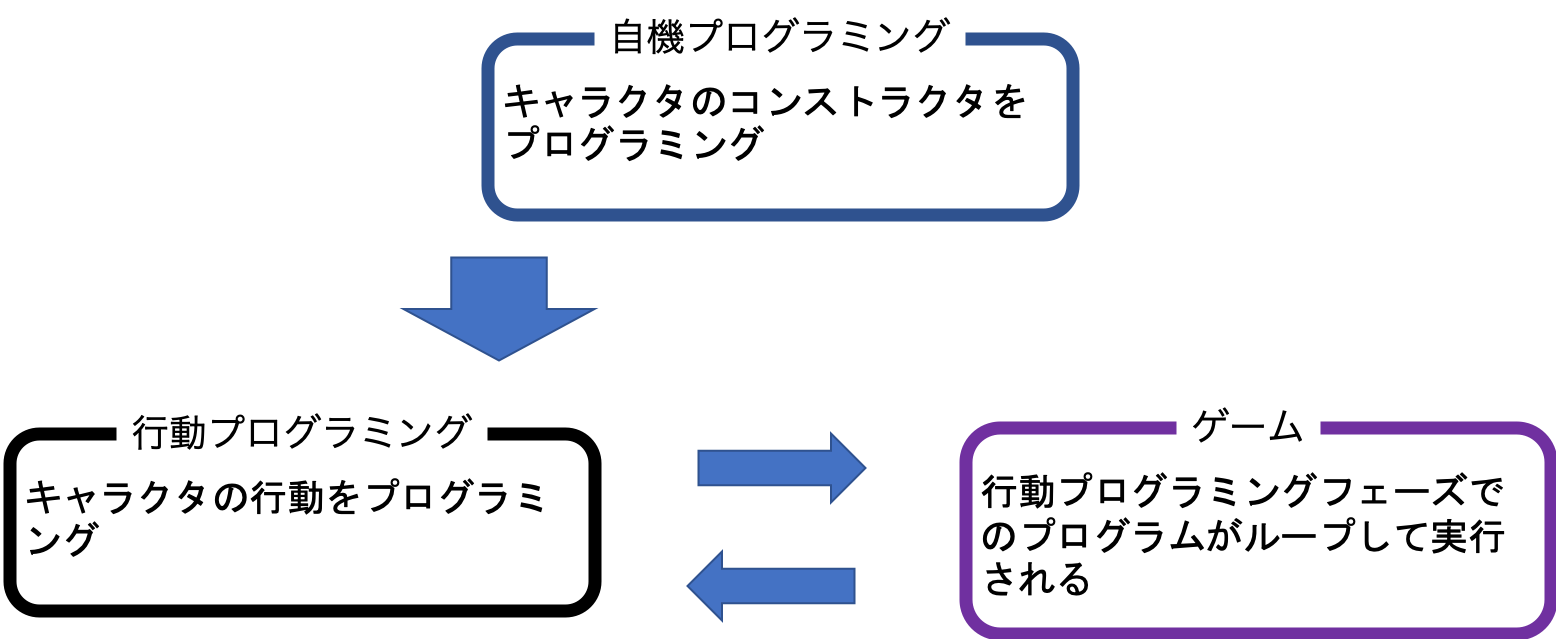
\includegraphics[width=1.0\linewidth]{image/phase.eps}
  \end{center}
    \vspace{-8mm} 
  \caption{フェイズ遷移図}
  \label{phase}
\end{figure}

\subsubsection{自機プログラミングフェイズ}
プレイヤが「vsPlayer」モードを選んで相手プレイヤとマッチングする,または「vsComputer」モードを選ぶとこのフェイズに移行する.プレイヤには1か2の番号が振られ,番号に応じて画面の背景色や制御するキャラクタの番号が異なる.このフェイズの様子を図\ref{characterProgramming}に示す.

ここでは予めエディタにプレイヤが操作するキャラクタのコンストラクタが記述されており,プレイヤはパラメータを書き換えることができる.具体的なパラメータにはappearance,life,clock,powerがある.appearanceはキャラクタの外見であり,文字列を指定できるため,絵文字などを使ってプレイヤの好きな見た目を選ぶことが可能である.lifeはキャラクタの体力であり,いわゆるHP(ヒットポイント)を表している.非負の整数を指定でき,この値が0以下になるとプレイヤはゲームに敗北する.clockはキャラクタが行動できる回数の多さを表しており,非負の整数を指定できる.プレイヤは後述する行動プログラミングフェイズにおいて自分のキャラクタを制御するプログラムを記述し対戦するが,その際に記述したプログラムは10秒間ループして実行される.このループのインターバルを決めるのがclockであり,値が大きいほどインターバルは短くなる.powerはキャラクタの攻撃力を表しており,これも非負の整数を指定できる.この値が大きいほど,自分が操作するキャラクタの攻撃が相手キャラクタに命中した際に削るlifeの値が大きくなる.双方のプレイヤが各パラメータを記述し終わると次の行動プログラミングフェイズに移行する.

\begin{figure}[!ht]
  \begin{center}
    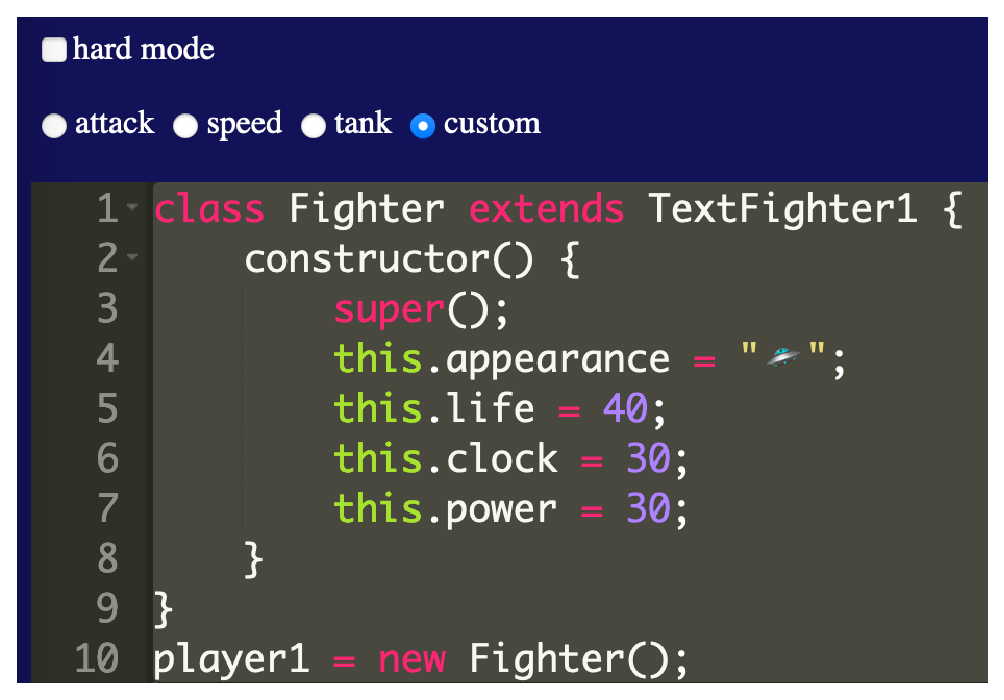
\includegraphics[width=1.0\linewidth]{image/characterProgramming.eps}
  \end{center}
    \vspace{-8mm} 
  \caption{自機プログラミングフェイズの様子}
  \label{characterProgramming}
\end{figure}

\subsubsection{行動プログラミングフェイズ}
このフェイズに進むと,自機プログラミングフェイズで記述したコンストラクタを元に両プレイヤが操作するキャラクタのインスタンスが作成され,ゲーム画面が表示される.このフェイズの様子を図\ref{actionProgramming}に示す.両プレイヤはプログラムをエディタに記述し,作成したキャラクタを操作する.エディタにはプレイヤに割り振られた番号に応じて「player1Loop」または「player2Loop」という名前の関数が予め用意されている.この関数が本フェイズ終了時にループして実行されることとなる.プレイヤは条件分岐や繰り返しなど従来のJavaScriptの文法の他に独自に用意されたプロトタイプメソッドを使うことができる.用意したメソッドにはキャラクタを移動するメソッド(moveUp(), moveDown(),randomMove())とキャラクタが攻撃を行うメソッド(shot())などがある.またプログラム内で各キャラクタのパラメータを参照することもできる.両プレイヤがプログラムを記述し終わると次のゲームフェイズに移行する.なおこのフェイズでは相手プレイヤがどのようなプログラムを記述しているかを見ることはできない.

\begin{figure}[!ht]
  \begin{center}
    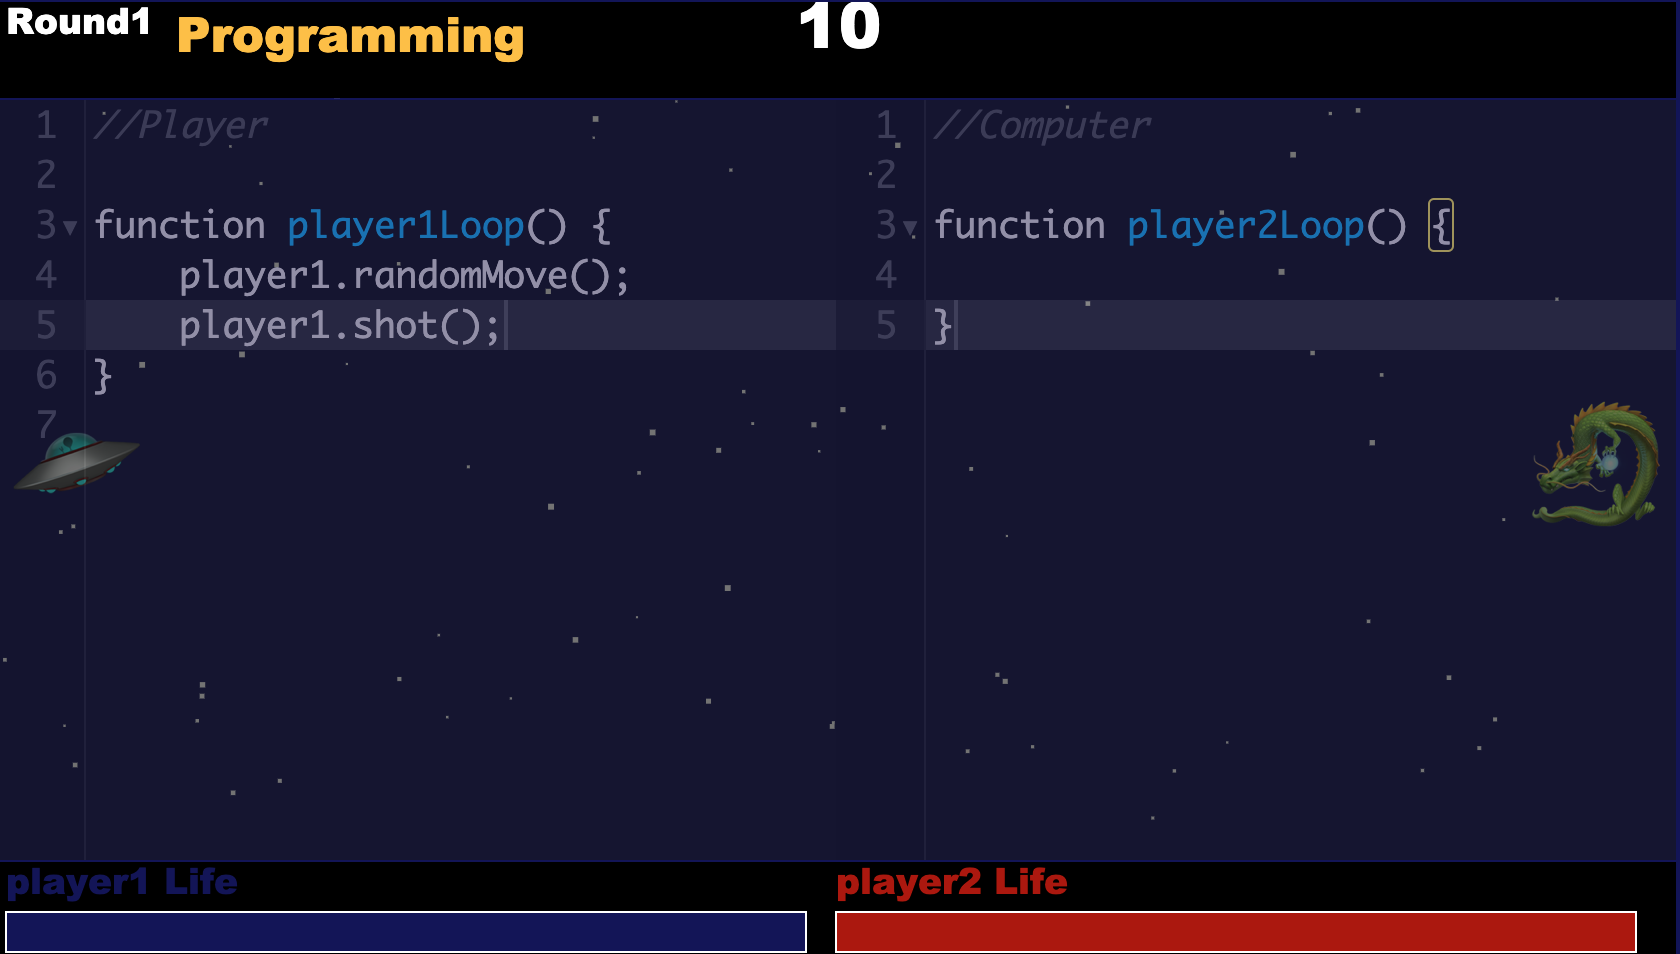
\includegraphics[width=0.6\linewidth]{image/actionProgramming.eps}
  \end{center}
    \vspace{-8mm} 
  \caption{行動プログラミングフェイズの様子}
  \label{actionProgramming}
\end{figure}

\subsubsection{ゲームフェイズ}
このフェイズでは行動プログラミングフェイズで記述したプログラムが10秒間ループして実行され,ゲームが進行する.このフェイズの様子を図\ref{game}に示す.このフェイズに移行した段階で,両プレイヤは相手プレイヤが記述したプログラムを閲覧することができる.このフェイズにおいて相手キャラクタを攻撃し,lifeの値を0以下にしたプレイヤの勝利となる.勝敗が決まらない場合はプログラム終了時の各パラメータを引き継いだまま行動プログラミングフェイズに戻り,再度プログラミングしゲームフェイズに移行するという過程を勝敗が決まるまで繰り返す.

また画面の下には擬似的なコンソールを配置しており,プログラムの実行時に発生したエラーが表示されるため,開発者ツールを開かずとエラーを確認できるようになっている.

\begin{figure}[!ht]
  \begin{center}
    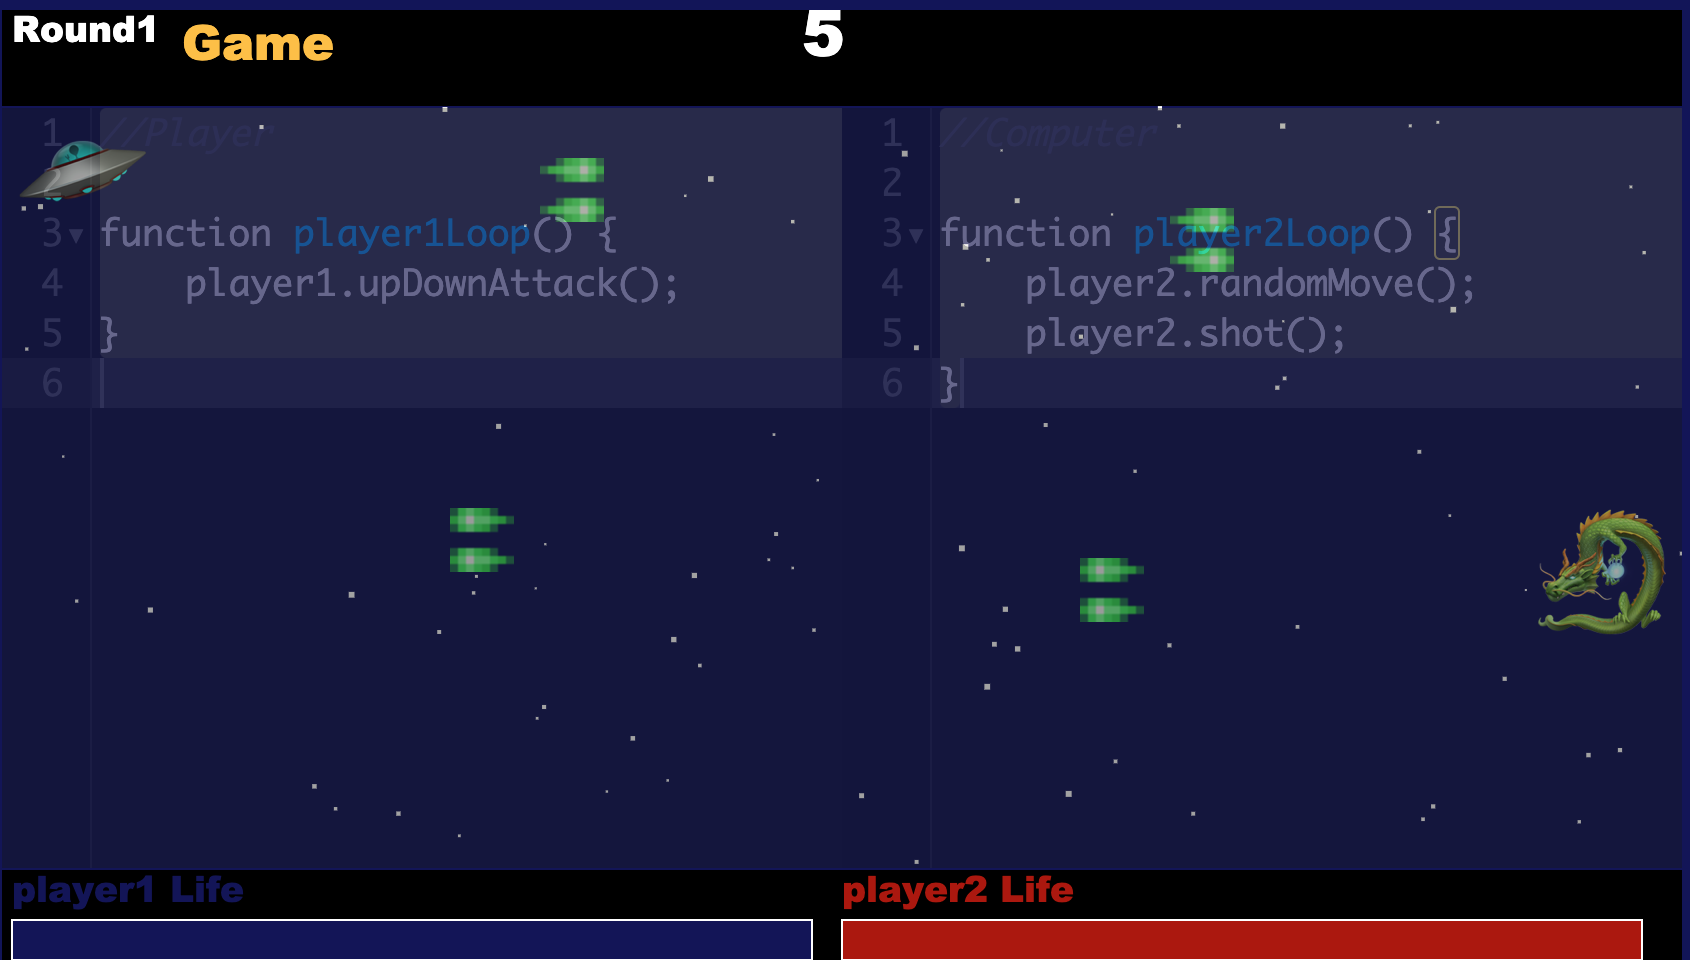
\includegraphics[width=0.8\linewidth]{image/game.eps}
  \end{center}
    \vspace{-8mm} 
  \caption{ゲームフェイズの様子}
  \label{game}
\end{figure}

\subsection{評価実験}
提案システムの使用・観戦に関する感想や影響,その用法を調査するために評価実験を実施した.システムを用いて対戦するプログラマと対戦を観戦するプログラミング初学者を集め,システムでの対戦と観戦を実施し,アンケート調査と実際に対戦で使用されたプログラムのログを分析することでシステムを評価した.

\subsubsection{実験参加者}
実際にゲームをプレイするプログラマとしては,プログラミング(主にオブジェクト指向言語)の経験が3年以上ある大学院生2名(男性)に声をかけた.2名とも日常的にアクションやシューティング等のジャンルのゲームをプレイするため,システムをプレイする際にゲームに不慣れなためハンデが生まれることはないと思われる.また両者とも3年以上JavaScriptを使用した経験がある.

またプレイを観戦するプログラミング初学者は,国際人間科学部にて開講されていた講義「プログラミング基礎演習1」の受講者を対象とした.受講者のうち,実験に参加した者は77名であり,うち37名が男性,40名が女性であった.またこの講義ではJavaScriptにおける変数,条件分岐,繰り返しなどの基礎的な文法を教えており,実験参加者は実験を行う時点でこれらを学習済であった.なお,うち23名は授業以前にプログラミングを学習した経験があったが,プログラミングによってソフトウェア開発を行った経験のある者はいなかった.

またプログラマ含む実験参加者の全員が,競技プログラミングやプログラミングゲームなどのプログラミングを題材としたエンタテインメントシステムを使用した経験がなかった.

\subsubsection{実験内容}

初めにプログラマ2人にプログラミングやゲームの経験に関する簡単な事前アンケートを行った後,提案システムにある程度慣れ,用法を理解してもらう必要があるため,システムの練習をするための期間を設けた.システムの使用方法,ゲームシステム,独自に用意したメソッドなどについて説明した後,11/13から11/19の1週間システムを自由に使用させた.また,ただシステムを使用させただけではゲームに対する理解が深まらない可能性があるため,期間中に2つのタスクをこなさせた.1つは1人以上とシステムを使った対人戦を行うことであり,もう1つは相手がランダムな戦略を実行してくる対CPU戦において,勝率が高いと考えられるプログラムを作成することである.

なお期間中はシステムに関する意見・疑問を逐次報告させ,システム使用における問題を改善した.またプログラマがシステムを使用する際に利用するWebブラウザはGoogle Chromeに統一した.

練習期間が終わった翌日に,プログラマ同士の対戦を行った.対戦はシステムに関するプログラマ同士のコミュニケーション等の所作を観察するため,感染症対策を徹底した環境で対面にて行った.両者の対戦時の画面を録画し,対戦後にシステムに関する事後アンケートを行った.なお練習期間中・対戦中にプログラマが記述した全てのコードのログを収集した.

そして「プログラミング基礎演習1」の最終講義で受講者に事前アンケートを行った後,初学者が観戦しやすいように対戦動画を編集したものをzoomを介して閲覧させた.またその後にシステムに関する事後アンケートを行った.

\subsubsection{アンケート結果}

対戦を観戦したプログラミング初学者に対する事後アンケートの内容及び結果を表\ref{interview}に示す.このアンケートに回答したのは実験参加者のうち74名であった.

\begin{table}[h]
  \begin{center}
    \caption{初学者に対する事後アンケート結果}
    \label{beginner_interview}
      \begin{tabular}{|c|c|c|c|c|c|c|c|} \hline
        \multirow{2}{*}{Q} & \multirow{2}{*}{質問項目} & \multicolumn{5}{c}{評価分布} & \multirow{2}{*}{平均} \\
        & & 1 & 2 & 3 & 4 & 5 & \\ \hline\hline
        Q1 & ゲームを観戦するのは楽しかったか & 3 & 6 & 33 & 27 & 5 & 3.34\\ \hline
        Q2 & ゲームの出力はプログラムを理解する助けになったか & 0 & 9 & 25 & 30 & 10 & 3.55\\ \hline
        Q3 & 観戦によってプログラミングに対する興味関心は高まったか & 1 & 11 & 23 & 33 & 6 & 3.43\\ \hline
        Q4 & 観戦によってプログラミングに関する理解が深まったか & 1 & 23 & 29 & 17 & 4 & 3.00\\ \hline
      \end{tabular}
      \\(1:全くそう思わない, 5:とてもそう思う)
  \end{center}
\end{table}

まずゲーム観戦の楽しさに関して(Q1)であるが,実験参加者の多くが肯定的な回答を示した.またキャラクタが攻撃,移動するなどのゲームの出力がプログラム理解の助けになったかという質問(Q2)に関しても3以上の評価が多かった.また観戦によりプログラミングに対する興味関心が高まったかという質問(Q3)についても,3以上の回答が多くなった.また観戦によってプログラミングに関する理解が深まったかという質問(Q4)に関しては,やや低い評価が多い結果となった.またこれら意外にも以下の質問をした.

\begin{itemize}
  \item Q5.このゲームを実際にプレイしたいか(プレイしたい/プレイしたくない)
  \item Q6.このゲームに他にどのような機能が欲しいか
  \item Q7.このゲームに関する意見
\end{itemize}

まずこのゲームを実際にプレイしたいかという質問(Q5)に関しては64.9\%がプレイしたいと回答した.またこのゲームに他にどのような機能が欲しいかという質問(Q6)に関しては「色んな技が繰り出せるような機能」「通常攻撃以外にため技のようなものが欲しいと思った」「回復アイテム的なものや必殺技」「攻撃を受けたときの衝撃波」などの回答があり,キャラクタの行動,エフェクト,アイテムの概念の追加などを求める意見が多く見られた.また「プログラム内容を解説する機能が欲しい」という意見も複数あり,Q4の結果にも見られるように,プログラムの内容をより分かりやすくする工夫が必要だと考えられる.またこのゲームに関する意見(Q7)としては,「自分のプログラミングのレベルを上げたいと思った」「面白い」「プログラミングを楽しみながら学習できると言う点でとても面白いと感じた」などゲームに対する肯定的な意見が多く得られた.

しかし「プログラミング初心者には少し難しかった」「楽しめるようになるまでのハードルが高そうだった」「今持っている知識では自分では動かすことが出来ないと感じた」など現状の自分のプログラミングスキルではゲームをプレイするのは難しそうに感じる反応も多く得られた.

またシステムをプレイしたプログラマにも同様に事後アンケートを行った.その内容・結果を表\ref{interview}に示す.

\begin{table}[!ht]
  \centering
  \caption{プログラマに対する事後アンケート結果}
  \label{programmer_interview}
    \begin{tabular}{|c|c|c|c|} \hline
      \multirow{2}{*}{Q} & \multirow{2}{*}{質問項目} & \multicolumn{2}{c}{プログラマ} \\ 
        & &A&B\\ \hline\hline
      Q1 & システムをプレイするのは楽しかったか & 4 & 5 \\ \hline
      Q2 & ゲームの出力はプログラムを理解する助けになったか & 4 & 5\\ \hline
      Q3 & プレイすることでプログラミングに対する興味関心は高まったか & 3 & 5\\ \hline
      Q4 & プレイによってプログラミングに関する理解が深まったか & 1 & 3\\ \hline
    \end{tabular}
    \\(1:全くそう思わない, 5:とてもそう思う)
\end{table}
この結果についても初学者に対する事後アンケートと同様の傾向があり,Q1,Q2,Q3については肯定的な評価が得られたが,Q4に関しては相対的に評価が低かった.またそれら以外にも以下の質問をした.

\begin{itemize}
  \item Q5.累計何時間程度システムを使用したか
  \item Q6.ゲームの難易度は自分にとって適切だったか
  \item Q7.どのような点が簡単(難しい)と感じたか
  \item Q8.ゲームに他にどのような機能が欲しいか
  \item Q9.今後もこのゲームを使用したいか
  \item Q10.ゲームに関する意見
\end{itemize}

累計何時間程度システムを使用したかという質問(Q5)に関しては1名が2時間,1名が6時間と回答した.またゲームの難易度は自分にとって適切だったかという質問(Q6)に関しては1名が適切だった,1名がやや難しかったと答えた.具体的には(Q7)「リファレンスが乏しくプログラムを書きづら買った」「現状のシステムではある程度システムを使い込んだ人をを想定した作戦を立てづらかった」と回答した.ゲームに他にどのような機能が欲しいかという質問(Q8)に対しては,「オブジェクトが持っている値を確認できるリファレンスのようなものが欲しい」「横移動ができれば,被弾しやすいリスクと引き換えに,敵が来そうな位置で敵より先に弾を打ち込めるチャンスが増える」と回答していた.また今後もこのゲームを使用したいか(Q9)という質問には2名とも「使用したい」と回答した.なおゲームに関する意見は「相手のコードを読んで対処するという部分をもっと積極的にするべきだったかもしれない.ただし,相手の位置に近づくようにプログラムすれば確実に自分が先に被弾するので,自分は動かずに相手が近づくのを待つプログラム以外最良の手がないようにも思う.」というものが得られた.

\subsubsection{コードログ分析結果}

練習期間中・対戦中にプログラマが記述したプログラムのログ,提出したプログラムを分析することで,システムがどのように利用されているか,どのようなプログラムが記述されているかを調査した.分析手法としては各プログラムをパースし,プログラム中のキーワードを抽出した.パーサにはJavaScriptパーサのデファクトスタンダードであるEspria\cite{esprima}を用いた.また各プログラムの可読性についても分析した.その指標としてThomas McCabeの循環的複雑度\cite{complexity}とSLOC(source lines of code)を用いた.循環的複雑度とはソフトウェア開発におけるソフトウェア測定法であり,プログラム中の分岐の数からプログラムの複雑さを算出する.SLOCはソースコードの行数を意味し,今回は空行やコメント行などを除いた値である論理LOCを用いた.またこれらのパラメータの算出にはJavaScript抽象構文木のソフトウェア複雑性分析ツールであるescomplex\cite{escomplex}を使用した.

\vspace{10truept}
\noindent
{\bf 対CPU戦におけるプログラム分析}

まずvsComputerモードで使用されたプログラムの分析結果について述べる.このモードで使用されたコードは合計327件である.全てのプログラムに含まれていたキーワード(演算子を除く)の個数をグラフ化したものを図\ref{vsComputer_keyword}に示す.もっとも多いキーワードはmyselfというものであるがこれは自キャラクタのインスタンスを代入するための変数として使われていた.プロトタイプシステムではプレイヤがplayer1になるかplayer2になるかがランダムに決定されていたため,それによってプログラムの内容を書き換えなくて済むように初めにmyselfに割り当てられたインスタンスを代入していたと思われる.次にplayer1というインスタンスを参照するキーワードが多く見られ,次いでインスタンスの座標を参照するキーワードであるy,条件分岐に用いられるifのキーワードが多く見られた.

プログラムの内容を観察するとキャラクタの座標を参照し,その値によって処理を分岐するプログラムが多く見られ,キーワードの分析結果と一致した.また「0x」で始まるキーワードがいくつか散見されるが,これはプレイヤが難読化ツールを用いてプログラムの難読化を試みた際に現れたキーワードである.

\begin{figure}[!ht]
  \begin{center}
    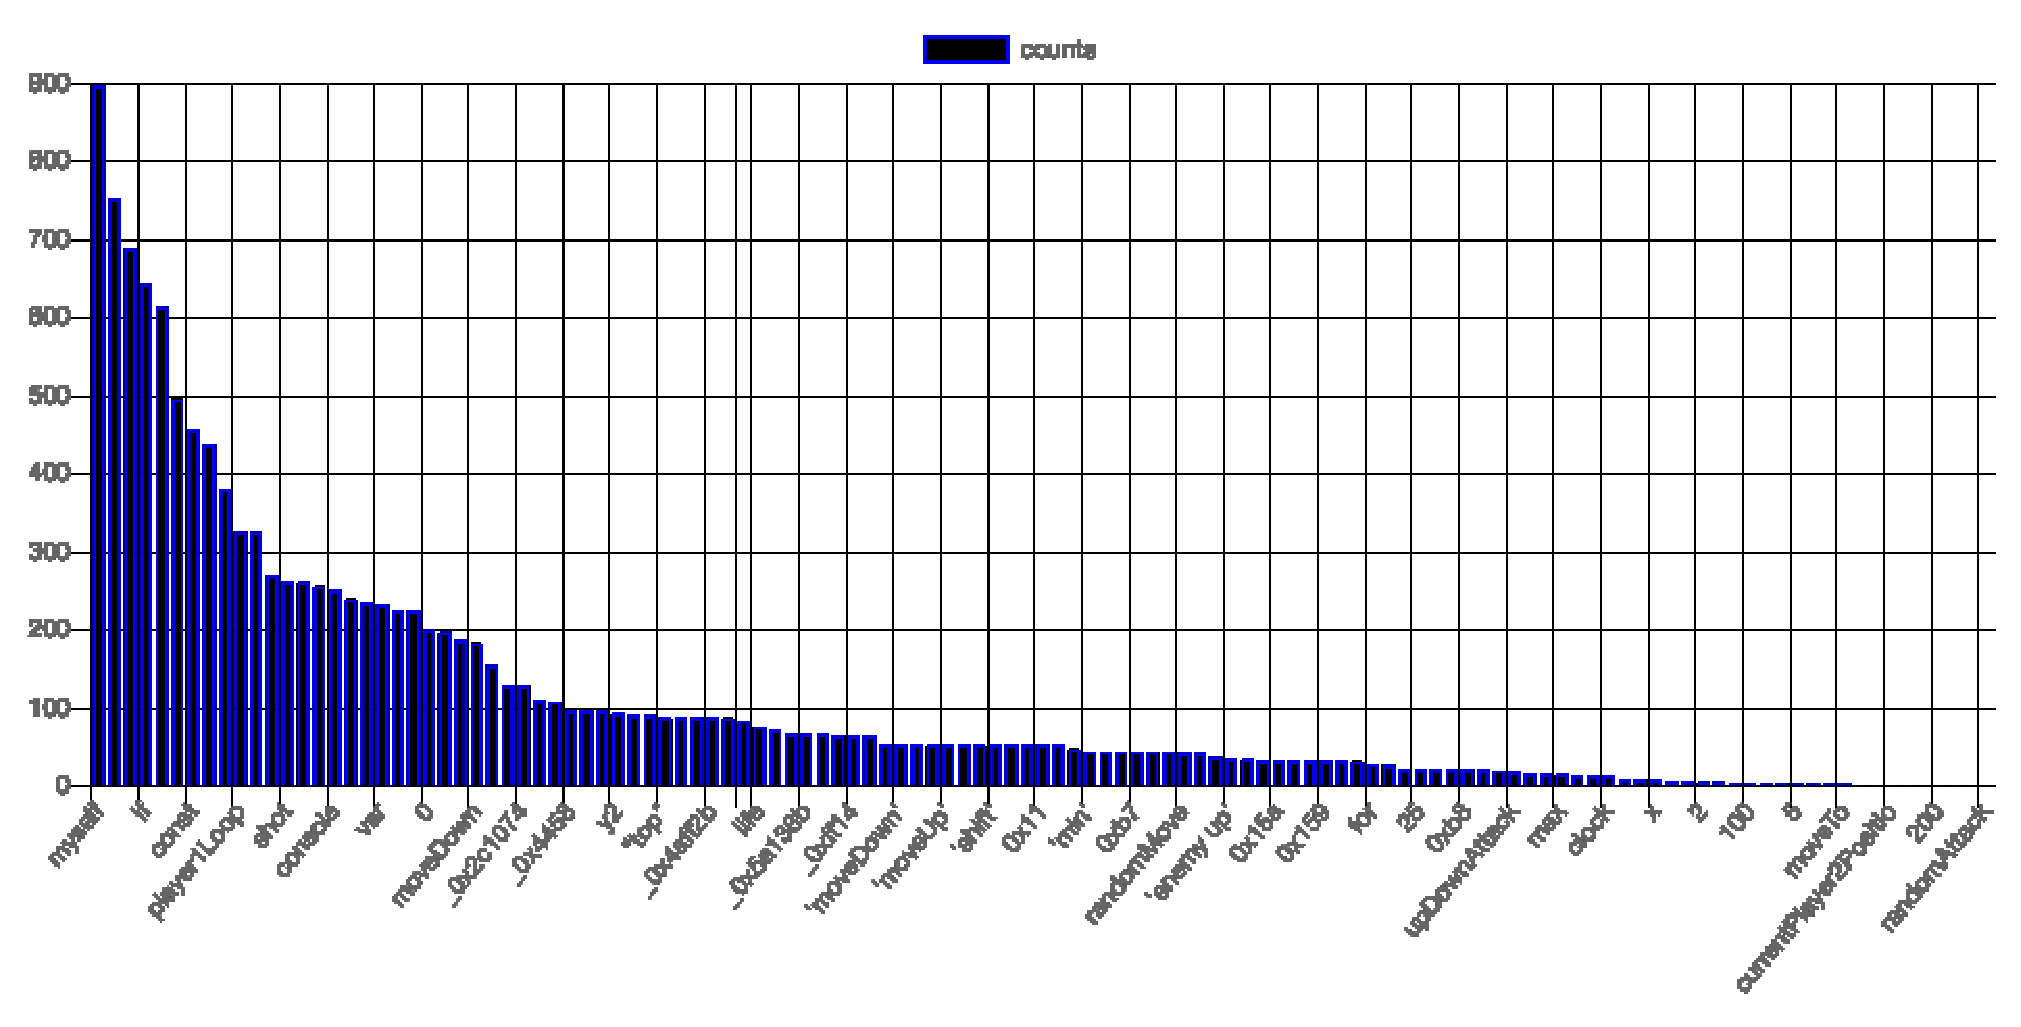
\includegraphics[width=1.0\linewidth]{image/vsComputer_result.eps}
  \end{center}
    \vspace{-8mm} 
  \caption{vsComputerにおけるキーワード分析}
  \label{vsComputer_keyword}
\end{figure}

次にvsComputerモードで投稿された各プログラムとSLOC・パラメータ数をグラフ化したものを図\ref{vsComputer_sloc_and_params}表示する.全体として徐々にSLOCが増加する傾向にあり,ゲームに習熟するほどコードの量が長くなっていったのだと考えられるが,無尽蔵にコードの量が増えていく傾向は見られなかった.しかし最大で30行前後のプログラムを初学者が短い時間で読解できるかは議論の余地がある.

またSLOCが平行線をたどり,パラメータの数が増加している部分はプレイヤが難読化ツールを使用した部分である.


\begin{figure}[!ht]
  \begin{center}
    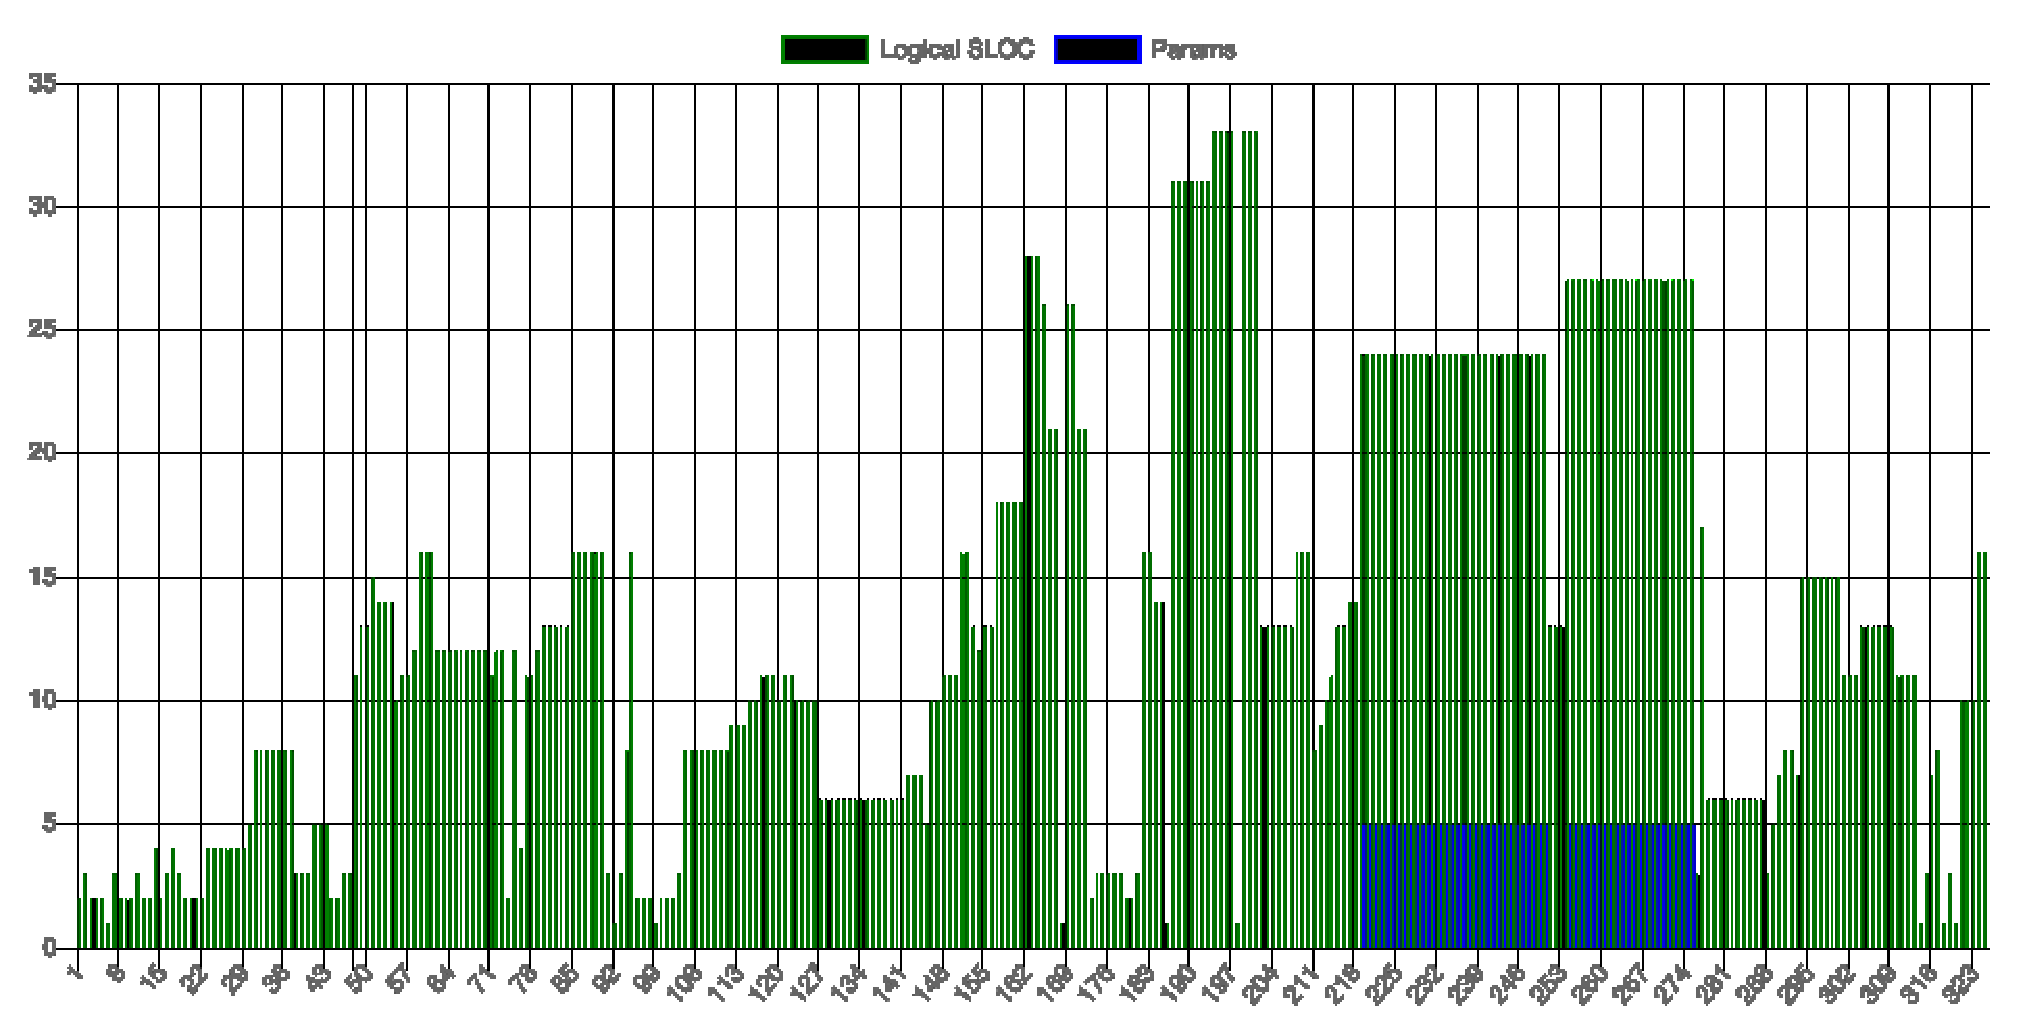
\includegraphics[width=1.0\linewidth]{image/vsComputer_escomplex_SLOC_params.eps}
  \end{center}
    \vspace{-8mm} 
  \caption{vsComputerにおけるSLOCとパラメータ数}
  \label{vsComputer_sloc_and_params}
\end{figure}

次にvsComputerモードにおける各プログラムごとの循環的複雑度を計測したグラフを図\ref{vsComputer_cyclomatic_complexity}示す.このグラフを観察すると各プログラムの循環的複雑度は概ね10以下に収まっていた.Thomasによると循環的複雑度が10を超えるプログラムはモジュール化などの工夫が必要であると述べられているため,今回分析したプログラムは分岐によりプログラムの可読性を大きく損なっていることはないと考えられるが,プログラムを実行する際に循環的複雑度が大きいと実行できないといったような制限を設け,プログラムの可読性が下がらないようにする工夫を設けても良いかもしれない.

\begin{figure}[!ht]
  \begin{center}
    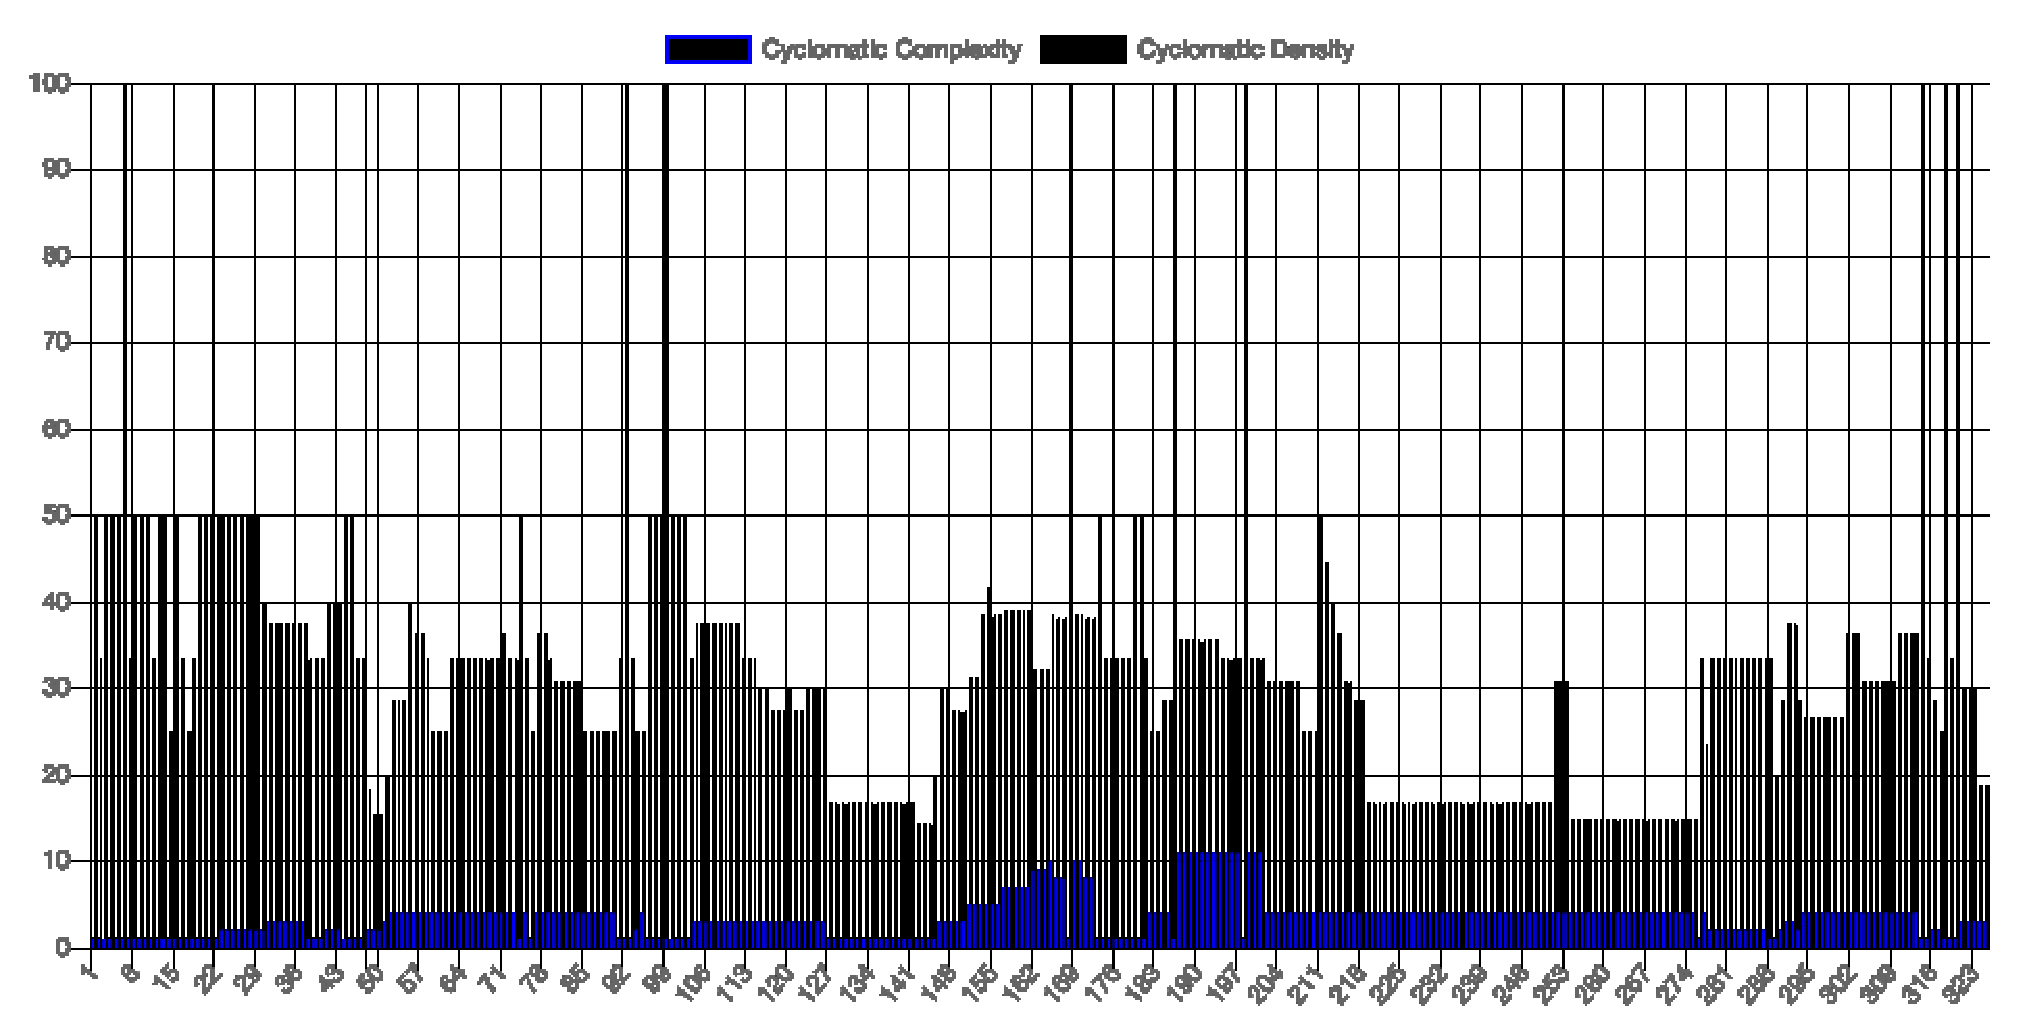
\includegraphics[width=1.0\linewidth]{image/vsComputer_escomplex_complexity.eps}
  \end{center}
    \vspace{-8mm} 
  \caption{vsComputerにおける循環的複雑度とその密度}
  \label{vsComputer_cyclomatic_complexity}
\end{figure}

\vspace{10truept}
\noindent
{\bf 対人戦におけるプログラム分析}

次にvsPlayerモード(対人戦)において使用されたプログラムの分析結果について述べる.このモードで使用されたコードは合計185件である.

全てのプログラムに含まれていたキーワード(演算子を除く)の個数をグラフ化したものを図\ref{vsPlayer_keyword}に示す.vsPlayerモードにおいて多かったキーワードは上からmyself,if,yであり,vsComputerモードと同様の傾向が見られた.プログラムの内容もvsComputerモードでのプログラムと大きく変わっておらず,対人戦で使用するプログラムをvsComputerモードで試していたと考えられる.

\begin{figure}[!ht]
  \begin{center}
    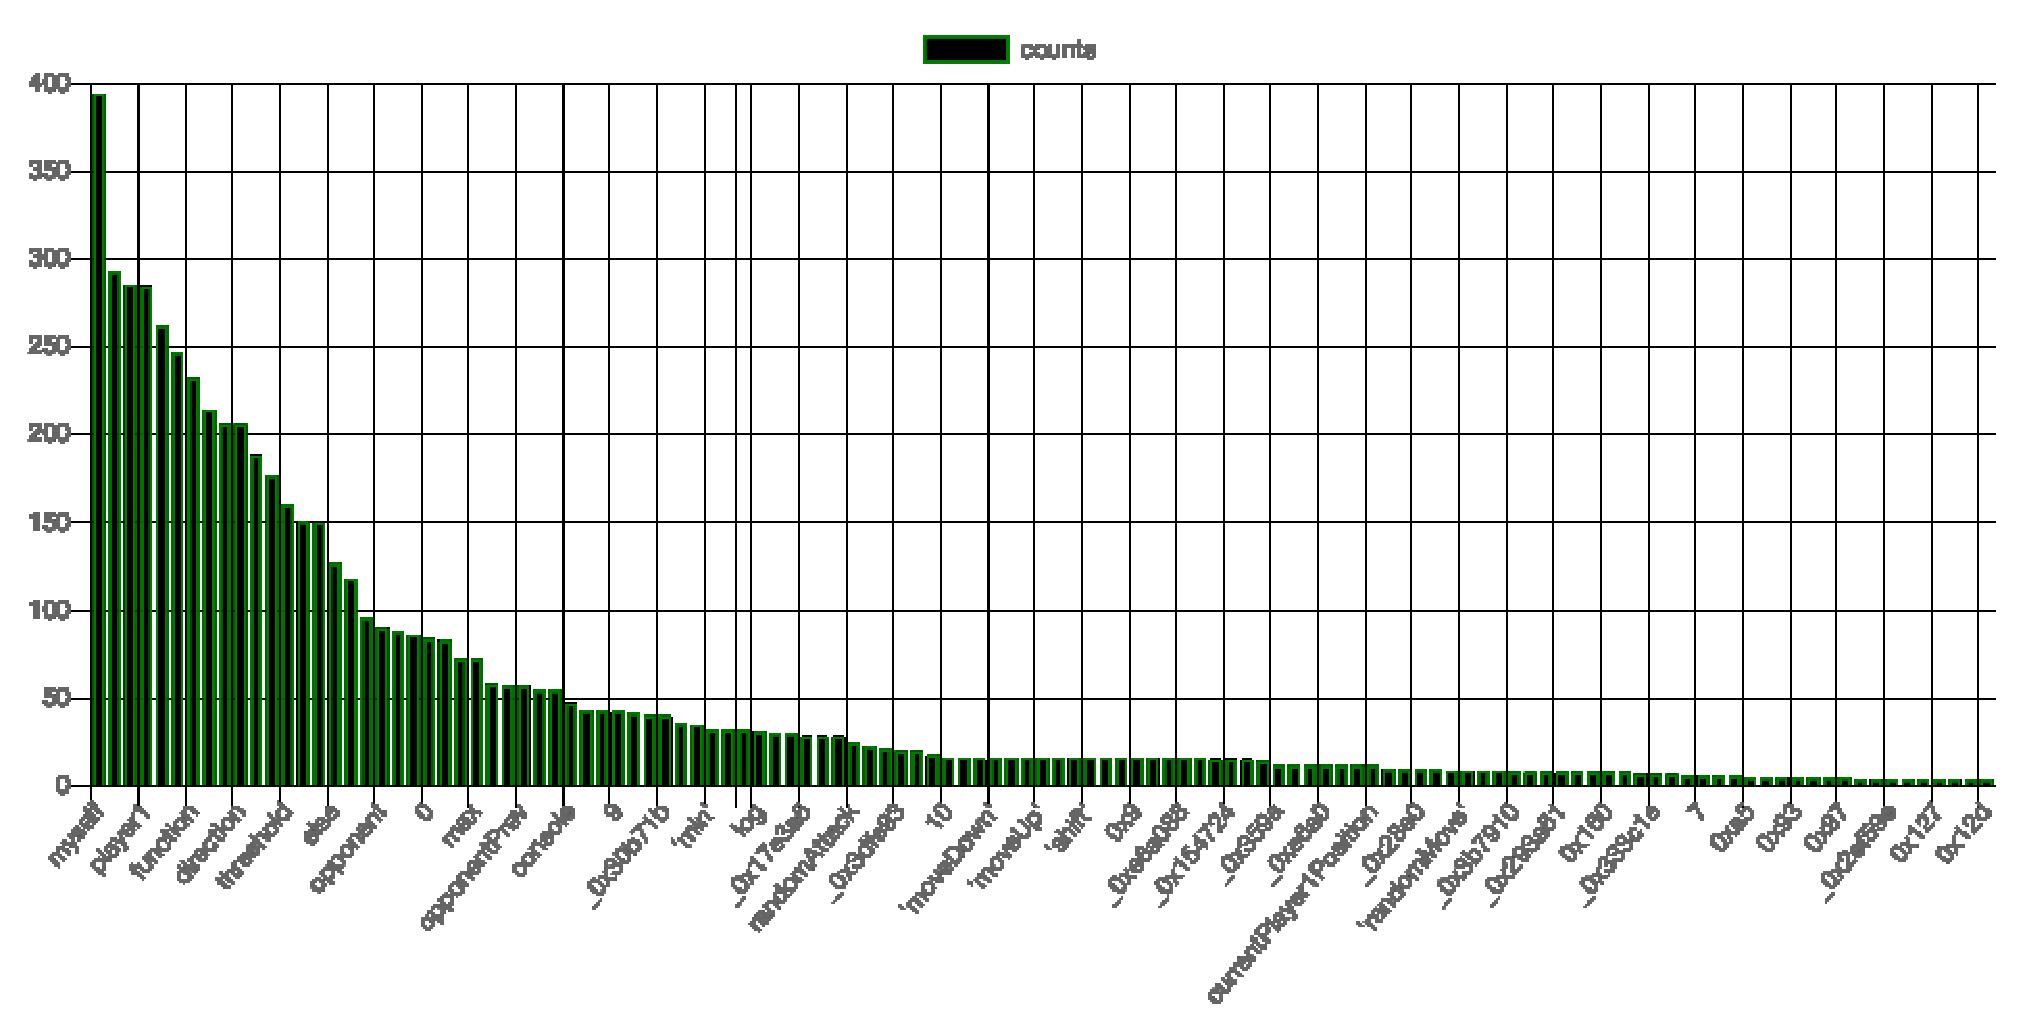
\includegraphics[width=1.0\linewidth]{image/vsPlayer_result.eps}
  \end{center}
    \vspace{-8mm} 
  \caption{vsPlayerにおけるキーワード分析}
  \label{vsPlayer_keyword}
\end{figure}

また各プログラムとSLOC・パラメータ数をグラフ化したものを\ref{vsPlayer_sloc_and_params}表示する.

\begin{figure}[!ht]
  \begin{center}
    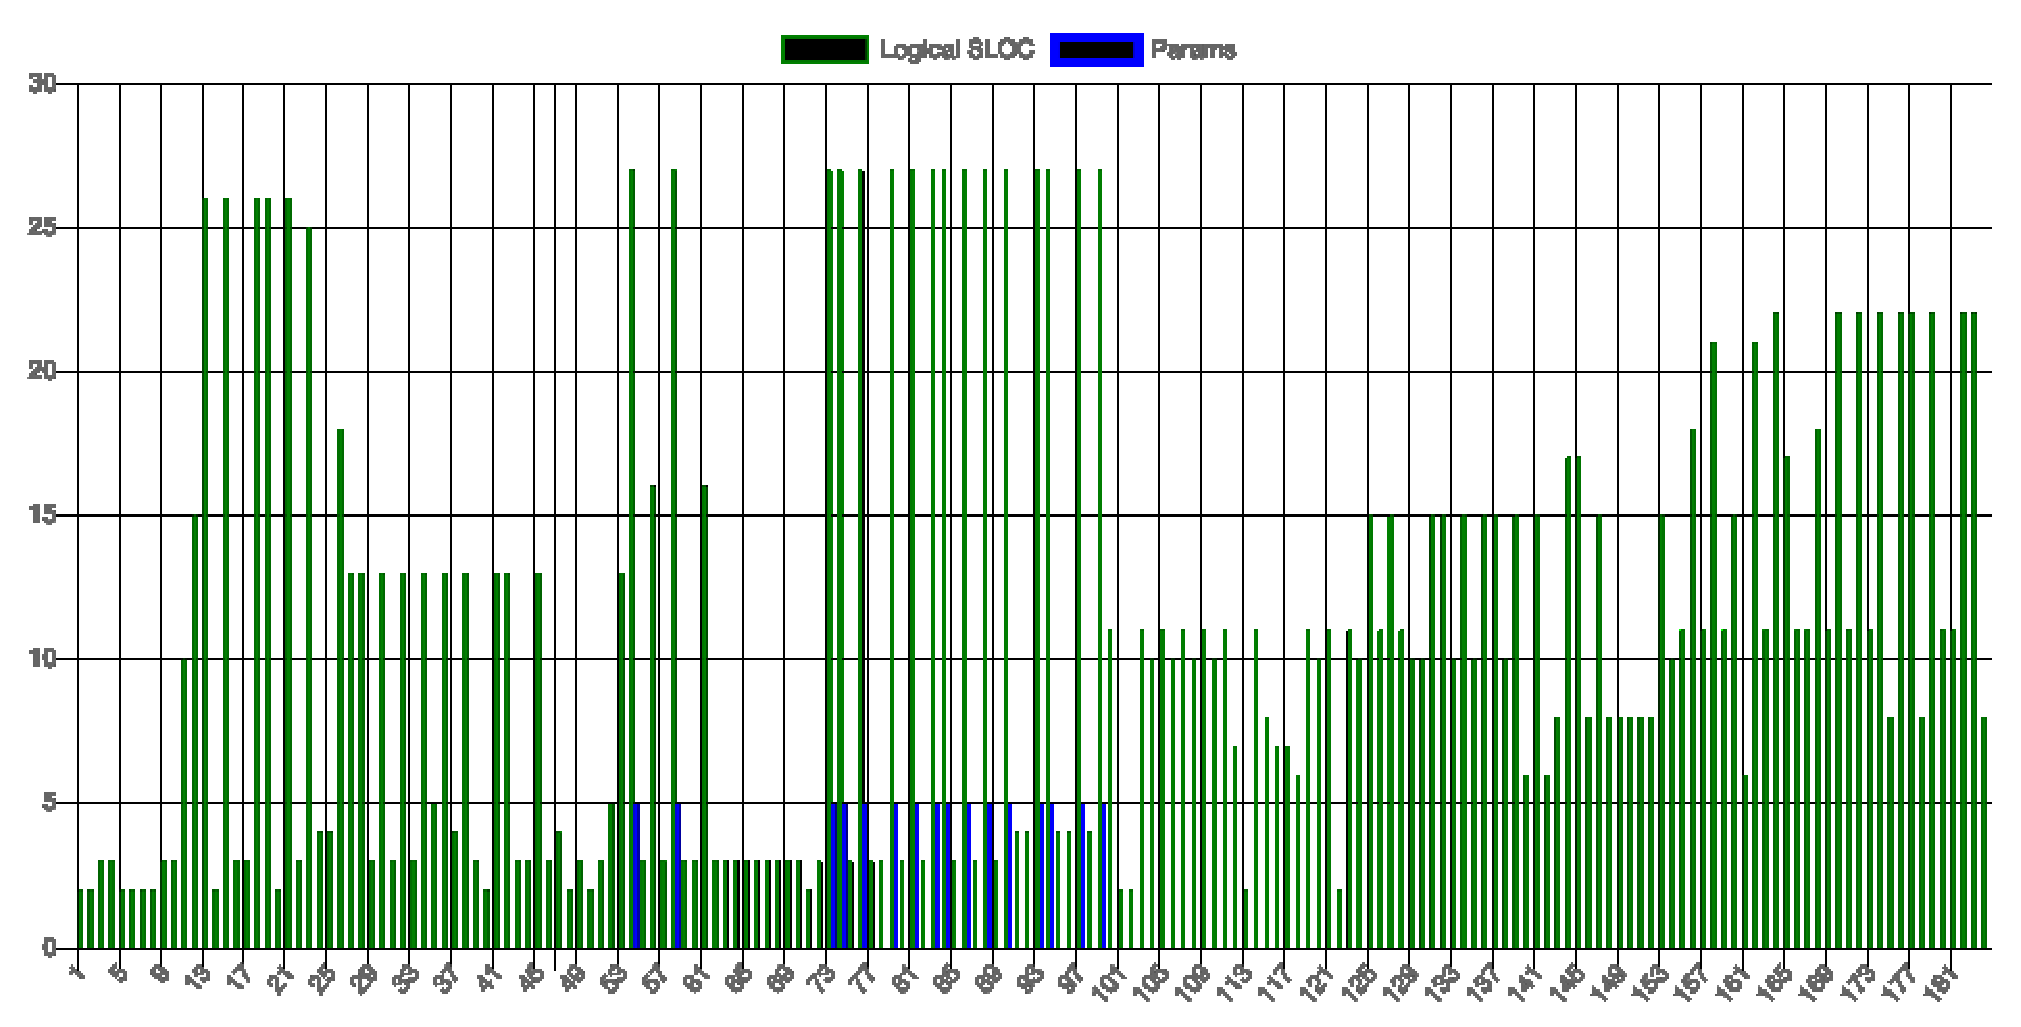
\includegraphics[width=1.0\linewidth]{image/vsPlayer_escomplex_SLOC_params.eps}
  \end{center}
    \vspace{-8mm} 
  \caption{vsPlayerにおけるSLOCとパラメータ数}
  \label{vsPlayer_sloc_and_params}
\end{figure}

次にvsPlayerにおける各プログラムの循環的複雑度を計測したグラフを図\ref{vsPlayer_complexity}示す.vsPlayerにおいても循環的複雑度の最大値は11であり,複雑な分岐はプログラム内に見られなかった.

\begin{figure}[!ht]
  \begin{center}
    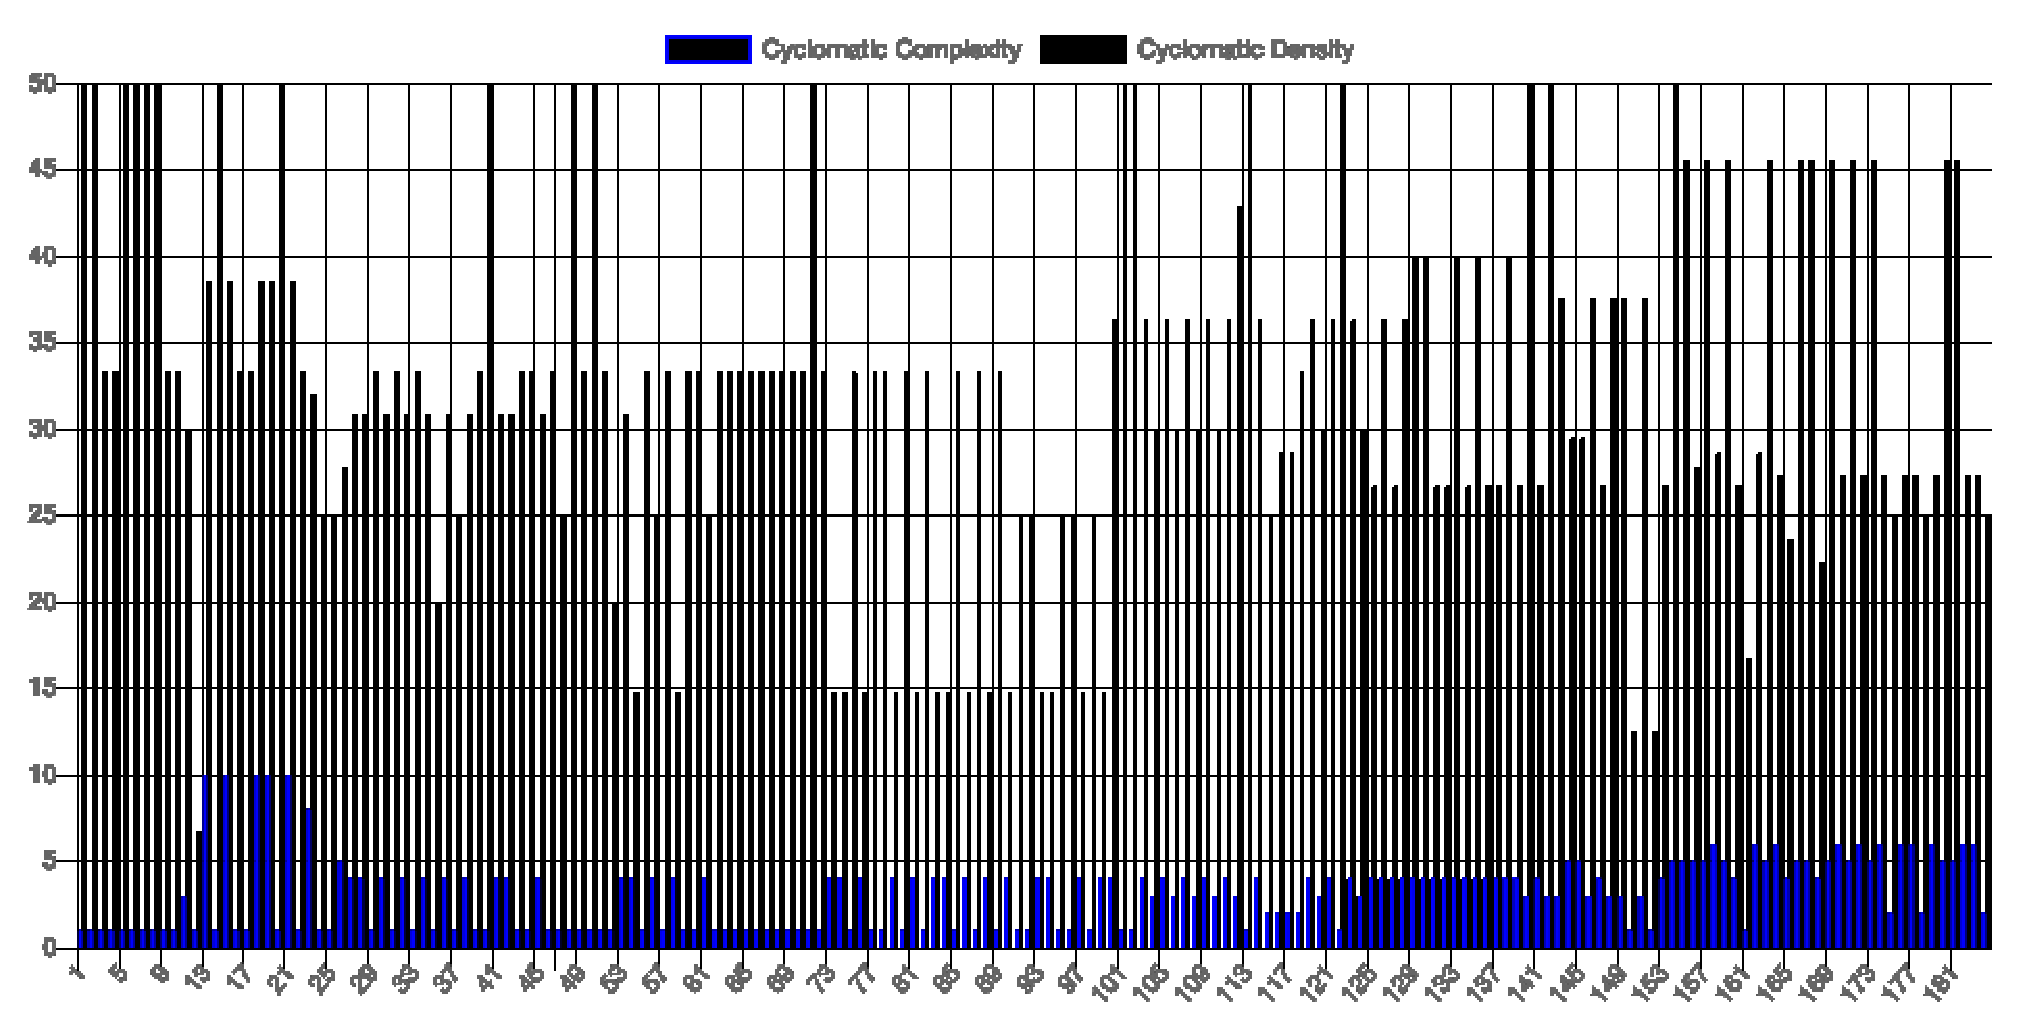
\includegraphics[width=1.0\linewidth]{image/vsPlayer_escomplex_complexity.eps}
  \end{center}
    \vspace{-8mm} 
  \caption{vsPlayerにおける循環的複雑度}
  \label{vsPlayer_complexity}
\end{figure}

\vspace{10truept}
\noindent
{\bf 提出プログラムの分析}

実験に参加したプログラマが提出したコードをソースコード\ref{mishima},\ref{shimizu}に示す.

\begin{lstlisting}[caption=プログラマA, label=mishima]
  const opponent = player1;
  const me = player2;
  let currentPlayer2Position = 240;
  let currentMyPosition = 240;
  function player1Loop() {
      if (currentPlayer2Position === currentMyPosition){
          currentMyPosition - 30 < 0 ? player1.moveDown() : player1.moveUp();
          player1.shot();
      } else {
          currentMyPosition < currentPlayer2Position ? player1.moveDown() : player1.moveUp();
          player1.shot();
      }
      
      currentPlayer2Position = player2.y;
      currentMyPosition = player1.y;
  }
\end{lstlisting}

プログラマAの記述したプログラムは,相手キャラクタと自キャラクタの位置関係によって処理を分岐している.大まかな戦略としては,相手キャラクタと自キャラクタの座標を比較し,同じ位置にいれば上あるいは下に動いて攻撃し,違う位置にいれば相手キャラクタのいる方向へ移動し攻撃する,というものである.

\begin{lstlisting}[caption=プログラマB, label=shimizu]
  const threshold = { min: -17-25, max: 9+25 };
  const myself = player1;
  const enemy = player2;
  function player1Loop() {
      var diff = enemy.y - myself.y;
      var direction = enemy.direction;
      console.log(diff);
      if (diff > threshold.min && diff <= threshold.max) {
          if (direction === "top") {
              myself.moveUp();
          } else if (direction === "bottom") {
              myself.moveDown();
          }
      } else {
          if (diff < threshold.min) {
              myself.moveUp();
          } else if (diff > threshold.max) {
              myself.moveDown();
          }
      }
      myself.shot();
  }
\end{lstlisting}

プログラマBのプログラムもプログラマAと同様,キャラクタの座標を用いた処理を行っているが,キャラクタの向きを表すパラメータであるdirectionも使用している.自キャラクタと相手キャラクタの座標の差分が閾値の範囲内であれば,相手のdirectionを参照して相手と同じ進行方向に移動し攻撃,自キャラクタと相手キャラクタのが大きく異なれば,相手キャラクタから逃げて攻撃するというものである.

初学者が読解するという観点から考えると,これらのプログラムはあまり長くなくネストも深くないため,認知的負荷はそれほど大きくないが数値を用いた条件分岐や三項演算子などは読解する際に慣れが必要なため,やや読解に労力を要すると考えられる.




\subsubsection{評価実験に関する考察}

評価実験に関する考察について述べる.プログラマ同士の対戦においては,行動プログラミングフェイズにおいて設定した相手のappearanceパラメータについて「かわいい」などとコメントする様子が見られた.また大戦後にお互いの記述したプログラムの内容や今までのプログラミング経験等に関するコミュニケーションが行われており,システムがコミュニケーションのきっかけを作ることができていた.また両者の対戦を観察した結果,プログラマがどういったプログラムを記述するか,どうプログラムを変更するかなどについて悩んでいる時間が多いため,リアルタイムな観戦においては,観戦者が飽きないように解説のような機能を入れたり,プログラミングする時間に制限を設けるなどの工夫が必要であると感じた.またプログラムの内容や戦略がやや一辺倒になってしまっていたため,1つの強い戦略が生まれてしまわないようにより多様なメソッドや強い戦法にリスクを持たせるなどして,多様な戦略を使わせる工夫をする必要があった.なおプログラマがプレイの際に開発者ツールのコンソールをしている様子が見られ,観戦する際にコンソールを使用している様子はやや初学者にとって内容が分かりづらくなるため,よりシステム画面上のコンソールの機能を拡充し,開発者ツールを使用せずとも対戦できるように設計したい.各々の対戦に着目すると,一方のプログラマの書いたプログラムが他方より圧倒的に強い場合は1ターンで決着がついてしまい,ターン性がうまく機能していない場合があったため,パラメータバランスを調整する必要がある.またプログラマの記述したプログラムを見ると,キャラクタの座標を用いた処理の際に数字を用いていたが,実際にプレイをしたことのない観戦者にとっては数字から具体的な座標をイメージするのが難しいため,極力不要な数値を用いずにプログラムできるように設計することが必要であると感じた.プログラムを開示する際により平易なプログラムに書き換えても良いかもしれない.

初学者の対戦の観戦においては,ライブでプログラマ同士が対戦している状況を用意することが困難であったため今回は動画を閲覧するという状況を用意したが,動画を見ただけでは実際に人が対戦しているという感覚が希薄であり,「プログラマがプログラミングしている」場面を見せるためには更なる工夫が必要であると感じた.

また今回の評価実験において,システムに対する肯定的な評価が得られたものの,どのような要素が初学者のプログラミングに対する興味に影響を与えていたのか,特に提案システムにおいて独特な要素であるリアルタイムな駆け引き・アドリブを誘発する要素の影響について調査する必要があると考えられる.

\subsection{課題}
提案システムの開発・評価実験で明確になった課題について議論する.大きく分けて「システムの改善(現状のプロトタイプをどう改善していくか)」と「今後の研究(今後どのように調査を進めていくか)」について述べる.

\noindent
{\bf システムの改善}

評価実験でのアンケート結果・コードログの分析結果を鑑みてより良いゲームデザインが必要であると感じた.まずパラメータバランスを調整し,1ターンで終わるなどすぐにゲームが終わって終わないようにする.またプレイヤ同士の対戦において圧倒的に力の差がある場合でも逆転できるような要素を加えることで,プレイヤ・観戦者がより楽しめるようにする.さらにこのゲームにおける強さがプログラマのスキルに比例し,かつ観戦者にとっても可読性の高いプログラムを表示できるよう,最大コード長に制限を設けたり,循環的複雑度の最大値に制限を儲けるなどの工夫を加える.またプロトタイプシステムではエラーを画面にそのまま表示するだけだったが,プレイヤを積極的にデバッグに向かわせる工夫を加える.これらの工夫に伴いUIを設計し直すとともにキャラクタのエフェクトも観戦に適切なものを採用する.またvsComputerモードでの対戦に,より戦略的なゲームAIを実装する予定である.さらにユーザログインを実装し,ランキング機能やGitHubアカウントを紐付けてプログラマ同士の交流を図るなどの機能も追加していきたい.

\noindent
{\bf 今後の研究}

今後はシステムに改善を咥えながらより多くのユーザを対象としたワークショップ・実験を行う.より多くの習熟したプログラマを対象とした調査だけでなく,初学者にもゲームをプレイさせ,初学者にとっての影響も調査する.プログラミング言語の基礎的な文法の理解を促すチュートリアルを実装し,プログラミング学習コンテンツとしての効果も調査していきたい.またライブでの対戦を初学者に観戦させ,本システムの特徴であるリアルタイム性・アドリブによる影響を重点的に調査する.なおどうすれば観客が内容を理解し,盛り上がることができるのかといったライブコーディングの見せ方についても調査を行う予定である.さらにリアルタイム性・アドリブが興味喚起に良い影響を及ぼしていたのなら,より若い世代に向けての興味喚起も可能かもしれない.ブロックベースでの制御や,ロボットなどフィジカルなものを制御する試みも行いたい.

今回はリアルタイムなシューティングゲームとしてシステムを実装したが,将棋の対戦に見られるようなプレイヤの熟考と解説者の解説を交えたプログラミングゲームも実現可能かもしれない.より幅広いジャンルのシステムを開発することで,プログラミング初学者向けコンテンツの拡充を目指す.




\newpage
\section{まとめ}

本論文では,テキストプログラミング言語によるプログラミング初学者の学習促進・興味喚起をするための2つのアプリケーションを提案した.

1つはクイズ,占いといったエンタテインメントを交えてGitHubにあるソースコードを初学者に読解させることでコードリーディングを促進するものであり,筆者の所属する研究室でケーススタディを行い,得られた問題点を改善したものをWebアプリケーションとして実装し直し,UWW2019にて議論を行った.結果,肯定的な反応が得られ,プログラミング言語への理解が深まったという意見が得られたり,プログラミングにまつわるコミュニケーションを促進できている様子が確認されたが,コードリーディングに対する抵抗感が強くなったといったネガティブな意見もあり,表示プログラムの選択アルゴリズムや継続的な利用を促す工夫など,いくつかの改善点が見つかった.

また2つ目のアプリケーションは,ライブコーディングのようなリアルタイム性・アドリブの要素を取り入れた対人形式のプログラミングゲームである.これを習熟したプログラマにプレイさせ,その対戦を初学者に観戦させることで初学者のプログラミングに対する興味関心を高めることを目指した.初学者を対象に評価実験を行った結果,肯定的な評価が多く得られ,初学者のプログラミングに対する興味喚起に成功したがゲームシステム・デザインに改善すべき点が見つかった.

今後はこの2つのシステムを通して得られた結果・意見を基に,ScratchやViscuitなどを用いてもプログラミングに対する興味を持てない層,特に高校生・大学生のプログラミング初学者を対象にプログラミングに楽しく取り組める学習コンテンツを拡充し,より広い層を対象にシステムの評価を行う.また本研究の結果を元に,より若い世代に対してのプログラミング学習システムの構築も視野に入れている. 

\newpage
\addcontentsline{toc}{section}{\protect\numberline{}{謝辞}}
\markright{}
\section*{謝辞}

本研究を行うにあたり,日頃より御指導,御激励を賜り,数々の御教示を頂きまし
た西田健志准教授に深甚なる謝恩の意を表します.また神戸大学大学院国際文化学研究科に在学中,御教示,御激励頂いた神戸大学大学院国際文化学研究科の諸先生方に感謝すると共に,諸職員の方々に感謝いたします.日頃より数々の御助言を下さいました諸先輩方,快適な環境を作って頂いた研究室の皆様方,実験に協力頂いた実験参加者の方々に深く感謝いたします.特にシステムの評価における多くのサポートを頂いた工学研究科の清水友順氏,国際文化学研究科の三嶋哲也氏に深く感謝いたします.

\newpage
\addcontentsline{toc}{section}{\protect\numberline{}{参考文献}}
\markright{}
\begin{thebibliography}{99}
	
	%はじめに
	\bibitem{survey}諸外国におけるプログラミング教育に関する調査研究, \url{https://www.mext.go.jp/a_menu/shotou/zyouhou/detail/__icsFiles/afieldfile/2018/08/10/programming_syogaikoku_houkokusyo.pdf}.
	\bibitem{guide}小学校プログラミング教育の手引(第三版), \url{https://www.mext.go.jp/content/20200218-mxt_jogai02-100003171_002.pdf}.
	\bibitem{matsumoto}松本絵里子 et al: C言語の概念と実行過程を可視化するプログラミング学習用アプリケーションの開発,専修ネットワーク&インフォメーション, No.24, pp.15--26 (Mar. 2016).
	\bibitem{okamoto}岡本雅子, 喜多 一: プログラミングの「写経型学習」における初学者のつまずきの類型化とその考察:, パイデイア: 滋賀大学教育学部附属教育実践総合センター紀要: memoirs of the Center for Educational Research and Training, Shiga University, 2014, 22, pp.49--53 (Mar. 2014).
	
	%コードリーディング関連
	\bibitem{progate}Progate, \url{https://prog-8.com/}.

	%GitHubを使った研究
	\bibitem{guzman}E.Guzman et al: Sentiment analysis of commit comments in GitHub: an empirical study, In Proceedings of the 11th Working Conference on Mining Software Repositories, 2014, pp. 352--355 (May. 2014).
	\bibitem{nagano}永野真知, 早瀬康裕, 駒水孝裕, 北川博之: GitHubとStackOverflowにおけるユーザ行動の統一的な分析, 情報処理学会第79回全国大会, pp. 363–364 (Mar. 2017).
	\bibitem{shibatou}柴藤大介, 有薗拓也, 宮崎章太, 矢谷浩司: CodeGlass:GitHubのプルリクエストを活用したコード断片のインタラクティブな調査支援システム, 情報処理学会インタラクション, vol.2019, pp.159–16 (Mar. 2019).

	%ゲーミフィケーションを使った研究
	\bibitem{ichinose}一ノ瀬智浩, 畑 秀明, 松本健一: ソースコード上の技術的負債除去を活性化させるゲーミフィケーション環境の開発, 情報処理学会関西支部支部大会講演論文集, vol.2016, (Sep. 2016).
	\bibitem{mitani}三谷将大, 寺田 実: Webアプリケーションによるゲーミフィケーションを用いたプログラミング上達支援システム, 第27回インタラクティブシステムとソフトウェアに関するワークショップ, (Sept.2018).

	\bibitem{tsutsui}筒井 優, 岩澤京子: 初心者向けオブジェクト指向プログラミング学習ゲームの開発, 第76回全国大会講演論文集, 2014, pp. 631--633 (Mar. 2014).

	% \bibitem{hikawa}樋川一幸, 松田滉平, 中村聡史: コミュニケーションチャネルに入り込む研究室実験BOTの提案と運用, 情報処理学会研究報告グループウェアとネットワークサービス,vol.3, pp. 1–7(Mar. 2019).

	%コードリーディングに関する研究
	\bibitem{omura}大村 裕, 渡部卓雄: プログラム理解のためのコードリーディング支援ツールの提案と実装, 日本ソフトウェア科学会講演論文集, vol.31, pp.44--446, (Sep. 2014).
	\bibitem{ishio}石尾 隆, 田中昌弘, 井上克郎: ソースコード上での情報タグ伝播によるコードリーディング支援, ウィンターワークショップ論文集, vol.2008, pp.31--32, (Jan. 2008).

	\bibitem{uww2019}Ubiquitous Wearable Workshop 2019, \url{http://cse.eedept.kobe-u.ac.jp/uww2019/}.

	%プログラミングゲーム関連

	%プログラミングを用いたエンタテインメント
	\bibitem{topcoder}Topcoder, \url{https://www.topcoder.com/}.
	\bibitem{codegolf}浜地慎一郎: Code Golf, \url{http://shinh.skr.jp/dat_dir/golf_prosym.pdf}.
	\bibitem{seccon}SECCON, \url{https://www.seccon.jp}.
	\bibitem{robocode}Robocode, \url{https://robocode.sourceforge.io/}.

	%プログラミング教育システム
	\bibitem{tpl}H.Tsukamoto et al: Programming education for primary school children usin a textual programming language, In 2015 IEEE Frontiers in Education Conference (FIE), pp. 1--7 (Oct. 2015).
	\bibitem{tsukamoto}H.Tsukamoto et al: Textual vs. visual programming languages in programming education for primary schoolchildren, 2016 IEEE Frontiers in Education Conference (FIE), IEEE, vol. 2016. p. 1--7 (Oct. 2016).
	\bibitem{scratch}M.Resnick et al: Scratch: programming for all, Communications of the ACM, 52(11), pp. 60--67 (Nov. 2009).
	\bibitem{viscuit}原田康徳: 子供向けビジュアル言語 Viscuitとそのインタフェース, 情報処理学会研究報告ヒューマンコンピュータインタラクション (HCI), vol. 2005, pp.41--48 (Nov. 2005).
	\bibitem{dolittle}S.Kanemune et al: Dolittle: an object-oriented language for K12 education, EuroLogo, vol. 2005, pp. 144--153 (Aug. 2005).

	%ライブコーディング環境
	\bibitem{livecodelab}LivecodeLab, \url{https://livecodelab.net/}.
	\bibitem{hydra}Hydra, \url{https://hydra.ojack.xyz/}.

	%プログラミングゲームを使った研究
	\bibitem{long}L.Ju: Just For Fun: using programming games in software programming training and education, Journal of Information Technology Education: Research, 2007, pp. 279--290 (Jan. 2007).
	\bibitem{joshua}J.Shi et al: Pyrus: Designing A Collaborative Programming Game to Promote Problem Solving Behaviors, Proceedings of the 2019 CHI Conference on Human Factors in Computing Systems, No. 656, pp. 1--12 (May. 2019).
	\bibitem{julian}J.Moreno: Digital competition game to improve programming skills, Journal of Educational Technology \& Society, vol. 15(3), pp. 288--297 (July. 2012).
	\bibitem{minakuchi}水口 充: 成績評価のためのプログラミングゲームの設計と実践, 研究報告エンタテインメントコンピューティング(EC), vol. 2016, pp. 1–7(July. 2016).

	\bibitem{mashitani}増谷海人, 赤澤紀子: 仮想現実を用いた初学者向けプログラミング学習システムの提案, 2018年度情報処理学会関西支部支部大会講演論文集,vol. 2018, (Sep. 2018).

	\bibitem{esprima}Esprima, \url{https://esprima.org/}.
	\bibitem{complexity} T.J.McCabe: A complexity measure, IEEE Transactions on software Engineering, vol. 1976, pp. 308--320 (Dec. 1976).
	\bibitem{escomplex}escomplex, \url{https://github.com/escomplex/escomplex}.

\end{thebibliography}


\end{document}